\documentclass[a4paper,11pt,twoside]{memoir}
\setcounter{secnumdepth}{2}
\let\STARTCODE\relax 
\let\STOPCODE\relax 
\STARTCODE
\usepackage{color,calc,graphicx,soul}
\definecolor{nicered}{rgb}{.647,.129,.149} \makeatletter
\newlength\dlf@normtxtw \setlength\dlf@normtxtw{\textwidth}
\def\myhelvetfont{\def\sfdefault{mdput}} \newsavebox{\feline@chapter}
\newcommand\feline@chapter@marker[1][4cm]{
  \sbox\feline@chapter{
    \resizebox{!}{#1}{\fboxsep=1pt
      \colorbox{nicered}{\color{white}\bfseries\sffamily\thechapter}
    }}
  \rotatebox{90}{
    \resizebox{
      \heightof{\usebox{\feline@chapter}}+\depthof{\usebox{\feline@chapter}}}
    {!}{\scshape\so\@chapapp}}\quad
  \raisebox{\depthof{\usebox{\feline@chapter}}}{\usebox{\feline@chapter}}
} \newcommand\feline@chm[1][4cm]{
  \sbox\feline@chapter{\feline@chapter@marker[#1]}
  \makebox[0pt][l]{
    \makebox[1cm][r]{\usebox\feline@chapter}
  }} \makechapterstyle{daleif1}{
  \setlength{\afterchapskip}{10pt}
  \renewcommand{\insertchapterspace}{}
  \renewcommand\chapnamefont{\normalfont\Large\scshape\raggedleft\so}
  \renewcommand\chaptitlefont{\normalfont\huge\bfseries\scshape\color{nicered}}
  \renewcommand\chapternamenum{} 
  \renewcommand\printchaptername{}
  \renewcommand\printchapternum{\vspace{-1.8cm}\null\hfill\feline@chm[2.5cm]\par}
  \renewcommand\afterchapternum{\par\vskip\midchapskip}
  \renewcommand\printchaptertitle[1]{\chaptitlefont\raggedleft
  	##1\par}
  \renewcommand\printchapternonum{\vspace{0.2cm}}
}

\makeatother
\chapterstyle{daleif1}
\STOPCODE
\usepackage[utf8x]{inputenc}
\usepackage[T1]{fontenc}
\usepackage[english, french]{babel}
\usepackage{lipsum}
\usepackage{lmodern}
\rmfamily
\DeclareFontShape{T1}{lmr}{b}{sc}{<->ssub*cmr/bx/sc}{}
\DeclareFontShape{T1}{lmr}{bx}{sc}{<->ssub*cmr/bx/sc}{}
\usepackage{epigraph}
\usepackage[french]{minitoc}
\setcounter{minitocdepth}{2}
\usepackage{soul}
\usepackage[pagebackref,colorlinks=true,citecolor=forestgreen,linkcolor=black,menucolor=alezan,urlcolor=prune]{hyperref}
\renewcommand*{\backref}[1]{}
\renewcommand*{\backrefalt}[4]{
\ifcase #1
-- Non cité.
\or
-- Cité page~#2.
\else
-- Cité pages~#2.
\fi}
\renewcommand*{\backrefsep}{, }
\renewcommand*{\backreftwosep}{ et~}
\renewcommand*{\backreflastsep}{ et~}
\usepackage{lingmacros}
\usepackage{fancybox}
\usepackage{pifont}
\usepackage{dsfont}
\def\sep{\begin{center}\begin{large}\ding{167}\end{large}\end{center}}
\renewcommand{\bibname}{Bibliographie}
\addto{\captionsenglish}{\renewcommand{\bibname}{Bibliographie}}
\addto{\captionsfrench}{\renewcommand{\listfigurename}{Liste des figures}}
\usepackage{newcent}
\usepackage{helvet}
\usepackage{color}
\usepackage{colortbl}
\usepackage{multirow}
\usepackage{longtable}
\newcommand{\withnofdp}[1]{{\NoAutoSpaceBeforeFDP #1}}
\usepackage{arydshln}
\usepackage{listings}
\lstset{
  language=XML, 
  basicstyle=\small,
  showspaces=false,
  showstringspaces=false,
  breaklines=true,
  breakatwhitespace=true,
  morecomment=[s]{<!--}{-->},
  alsoletter=.-,
  commentstyle=\itshape\color{gray},
  markfirstintag=true,
  string=[d]",
  keywords={correction},
  keywordstyle=\color{alizarine},
  stringstyle=\color{acier},
}
\usepackage{pgf,pgfarrows,pgfnodes}
\usepackage{tikz}
\usepackage{tikz-qtree}
\usepackage{tikz-dependency}
\usepackage{pgfplots}
\usetikzlibrary{mindmap,trees, backgrounds}
\usepackage{filecontents}
\usepackage{qtree}
\definecolor{acier}{HTML}{3A8EBA}
\definecolor{alezan}{HTML}{A76726}
\definecolor{alizarine}{HTML}{D90115}
\definecolor{amande}{HTML}{82C46C}
\definecolor{ambre}{HTML}{F0C300}
\definecolor{abricot}{HTML}{E67E30}
\definecolor{grey}{rgb}{0.9,0.9,0.9}
\definecolor{gris}{rgb}{0.1,0.1,0.1}
\definecolor{forestgreen}{rgb}{0.13,0.54,0.13}
\definecolor{dockerblue}{rgb}{0.11,0.56,0.98}
\definecolor{orange}{rgb}{0.64,0.16,0.16}
\definecolor{ocre}{HTML}{DFAF2C}
\definecolor{prune}{HTML}{811453}
\newcommand{\remCyril}[1]{\textcolor{dockerblue}{\emph{CG : #1}}}
\newcommand{\myex}[1]{\color{acier}{\emph{#1}}\color{black}}
\newcommand{\rg}[1]{\textsl{Remarque : #1}}
\def\euro{\mbox{\raisebox{.25ex}{{\it =}}\hspace{-.5em}{\sf C}}}
\newenvironment{changemargin}[2]{\begin{list}{}{
\setlength{\topsep}{0pt}
\setlength{\leftmargin}{0pt}
\setlength{\rightmargin}{0pt}
\setlength{\listparindent}{\parindent}
\setlength{\itemindent}{\parindent}
\setlength{\parsep}{0pt plus 1pt}
\addtolength{\leftmargin}{#1}
\addtolength{\rightmargin}{#2}
}\item }{\end{list}}
\usepackage{chngpage}
\usepackage{amssymb,amsmath,amsthm,amscd}
\usepackage{mathrsfs}
\usepackage{subfig}
\usepackage{tabularx}
\usepackage{calc}
\usepackage{graphicx}
\usepackage{hyperref}
\usepackage{makeidx}
\makeindex
\usepackage[french,intoc,refpage]{nomencl}
\renewcommand{\nomname}{Glossaire}
\renewcommand*{\pagedeclaration}[1]{\unskip\dotfill\hyperpage{#1}}
\makenomenclature
\newcommand{\nocontentsline}[3]{}
\newcommand{\tocless}[2]{\bgroup\let\addcontentsline=\nocontentsline#1{#2}\egroup}
%%%%%%%%%%%%%%%%%%%%%%%%%%%%%%%%%%%%%%%%%%%%%%%%%%%%%%%
%% EN-TETES ET PIEDS DE PAGE
\let\footruleskip\undefined
\usepackage{fancyhdr}
\pagestyle{fancy}% pour activer le style de pages personnalisé
\fancyhf{}%remise à zéro des en-tête et pied de page
\setlength{\headheight}{14pt} % pour fixer la hauteur de l'espace réservé à l'en-tête du haut

%%% Pas de numéro de page sur la première page des chapitres
\makeatletter
\let\ps@plain=\ps@empty
\makeatother

%===================== Style 1 =================================================
%En-tête : 
% * dans la boite de droite (R), pour les pages impaires (O)
% * et dans la boite de gauche (L), pour les pages paires (E)
% mettre le numéro de page (\thepage).
\fancyhead[RO,LE]{% 
\thepage
}
\fancyhead[LO]{\scshape \nouppercase{\rightmark}}  %%%Section
\fancyhead[RE]{\scshape \nouppercase{\leftmark}} %%% Chapitre 
\renewcommand{\headrulewidth}{.4pt}
\fancyfoot{}


%================================== Style 2 ====================================

% \fancyfoot[RO,LE]{% Boite de droite (R), pages impaires(O) et Boites de gauche pages paires
% \thepage
% }
% \fancyhead[CO]{\slshape \nouppercase{\rightmark}}  %%%Section
% \fancyhead[CE]{\slshape \nouppercase{\leftmark}} %%% Chapitre 
% \renewcommand{\headrulewidth}{.4pt}

% Remarques generales :
% nouppercase permet l'affichage en minuscules au lieu de majuscules
% slshape permet l'affichage en lettres penchés
% scshape permet l'affichage en petites capitales

% Pour que les pages paires sans texte (par exemple, à la fin d'un chapitre et
% avant un autre), ne contiennent ni en-tête ni pied de page (source :
% http://www.tex.ac.uk/cgi-bin/texfaq2html?label=reallyblank)
\let\origdoublepage\cleardoublepage
\newcommand{\clearemptydoublepage}{%
  \clearpage
  {\pagestyle{empty}\origdoublepage}%
}
\let\cleardoublepage\clearemptydoublepage

% Réglage fin des notes de bas de page
\FrenchFootnotes % pour les notes de bas de page à la française
\AddThinSpaceBeforeFootnotes % pour avoir une espace fine entre le mot et l'appel de note


%%%%%%%%%%%%%%%%%%%%%%%%%%%%%%%%%%%%%%%%%%%%%%%%%%%%%%%
%% CHAPITRE ETOILE
%% avec référence dans la table des matières et les bons en-têtes
%% il sert pour l'introduction, la page de notations.
\newcommand*\chapterstar[1]{%
  \chapter*{#1}%
  \addcontentsline{toc}{chapter}{#1}%
  \markboth{#1}{#1}}


%%%%%%%%%%%%%%%%%%%%%%%%%%%%%%%%%%%%%%%%%%%%%%%%%%%%%%%
% ENVIRONNEMENTS DE THEOREMES
\theoremstyle{plain} % style plain
\newtheorem{theo}{Théorème}[chapter]
\newtheorem{cor}[theo]{Corollaire}
\newtheorem{prop}[theo]{Proposition}
\newtheorem{lem}[theo]{Lemme}
\newtheorem{conj}[theo]{Conjecture}
\newtheorem*{theoetoile}{Théorème} % théorème non numéroté
\newtheorem*{conjetoile}{Conjecture} % conjecture non numérotée

\theoremstyle{definition} % style definition
\newtheorem{defi}[theo]{Définition}
\newtheorem{exemple}[theo]{Exemple}
\newtheorem{question}[theo]{Question}
\newtheorem{remarque}[theo]{Remarque}
\newtheorem{notation}[theo]{Notation}

% Pour renommer ``preuve'' en ``démonstration''
\renewcommand{\proofname}{Démonstration}


%%%%%%%%%%%%%%%%%%%%%%%%%%%%%%%%%%%%%%%%%%%%%%%%%%%%%%%
% ENVIRONNEMENTS DEDICACE ET EPIGRAPHE
\newenvironment{dedicace}{%
  \newpage\thispagestyle{empty}
  \hfill\begin{minipage}{100mm}\begin{flushright}\it}{%
  \end{flushright}\end{minipage}\vfill}

\newenvironment{epigraphe}{%
  \hfill\begin{minipage}{60mm}\begin{flushright}\footnotesize\it}{%
  \end{flushright}\end{minipage}\hspace*{7mm}\vfill}

\newcommand\tab[1][5mm]{\hspace*{#1}}
\parindent=0em
\begin{document}
\sloppy
\dominitoc
% ================================ Page du garde ==============================

\pdfbookmark[0]{Page de garde}{garde}
\thispagestyle{empty}

\begin{center}
  \begin{tabularx}{\textwidth}{m{10.3cm}m{4cm}}
	 
\includegraphics[width = 3.9cm]{z_images/0_logos/0_inalco.png} %% CG : 3.5cm au lieu de 3 cm
	&
        %% TODO: remplacer le logo du LIMSI par celui de la société ou
        %% du laboratoire où vous avez réalisé votre stage (si le
        %% sujet du mémoire de recherche fait suite à votre stage)
	 
\includegraphics[width = 3.9cm]{z_images/0_logos/1_inria.png} %% CG : 3.5cm au lieu de 3 cm
        \\ \hline
  \end{tabularx}
\end{center}

\begin{center}
\vspace{\stretch{1}}
% Permet de créer un espace vertical de longueur variable (\stretch) et de "poids" 1
{\Large \textbf{Institut National des Langues et Civilisations Orientales}}

\vspace{\stretch{1}}

{\normalsize Département Textes, Informatique, Multilinguisme}

\vspace{\stretch{2}}
\hrule
\vspace{\stretch{1}}
%% TODO: indiquez le titre de votre mémoire
{\LARGE \textbf{Titre du mémoire}}
\vspace{\stretch{1}}
\hrule

\vspace{\stretch{2}}

{\Huge \textsc{Master}}

\vspace{\stretch{1}}

{\LARGE \textsc{Traitement Automatique des Langues}}

\vspace{\stretch{1}}

{\normalsize \emph{Parcours~:}}

\vspace{\stretch{0.5}}

%% TODO: indiquez votre parcours
{\normalsize \emph{Ingénierie Multilingue}}

\vspace{\stretch{1}}

{\large par}

\vspace{\stretch{1}}

%% TODO: indiquez vos nom et prénom
\textbf{{\LARGE Martin \textsc{DIGARD}}}

\vspace{\stretch{2}}

{\normalsize \emph{Directeur de mémoire~:}}

\vspace{\stretch{0.5}}

%% TODO: indiquez le nom du/des directeur(s) de mémoire (enseignant
%% INaLCO qui supervise votre travail)
{\normalsize \emph{Damien NOUVEL}}

\vspace{\stretch{2}}

{\normalsize \emph{Encadrant~:}}

\vspace{\stretch{0.5}}

%% TODO: indiquez le nom du/des encadrant(s) de stage si votre mémoire
%% porte sur votre travail de stage
{\normalsize \emph{Florent JACQUEMARD}}

\vspace{\stretch{2}}

{\normalsize Année universitaire 2020-2021}

\end{center}

\cleardoublepage % pour laisser une page blanche au verso de la page de garde

\newpage
\setcounter{tocdepth}{1}
\pdfbookmark[0]{Table des matières}{tablematieres}
\tocless\tableofcontents
\newpage
\listoffigures
\listoftables
\printnomenclature
\newpage
%%%%%%%%%%%%%%%%%%%%%%%%%%%%%%%%%%%%%%%%%%%%%%%%%%%%%%%%%%%%%%%%%%%%%%%%%%%%%%%%%%


\chapter*{Introduction générale}
\adjustmtc
\addstarredchapter{Introduction générale} 
L’écriture musicale offre de nombreuses possibilités pour un rythme donné. Le contexte musical ainsi que la lisibilité d’une partition pour un batteur entraîné conditionnent les choix d’écritures. Reconnaître la métrique principale d’un rythme, la façon de regrouper les notes par les ligatures, ou simplement décider d’un usage pour une durée parmi les différentes continuations possibles (notes pointées, liaisons, silences, etc.) constituent autant de possibilités que de difficultés.\\Ce mémoire de recherche, effectué en parallèle d’un stage à l’Inria dans le cadre du master de traitement automatique des langues de l’Inalco, contient une proposition d’amélioration de Qparse, un outil de transcription et d’écriture automatique de la musique sur sa capacité à transcrire la batterie. Nous ne parlerons donc pas directement de langues naturelles, mais de l’écriture automatique de partitions de musique à partir de données audios. Cette exercice nécessitera la manipulation d’un langage musical codifié avec une grammaire (solfège, durées, nuances, volumes) et soulèvera des problématiques concernées par les techniques du traitement automatique des langues (TAL).\\
Nous proposons de rechercher des rythmes génériques (\textit{motifs}) en amont dans la chaîne de traitement. Les \textit{motifs} sont prédéfinis avec des combinaisons possibles (\textit{gammes}) qui leur sont associées. Ces \textit{motifs} et leur \textit{gammes} respectives sont appelés \textit{systèmes}. L’usage des \textit{systèmes} a pour objectif de fixer des choix le plus tôt possible dans la chaîne de traitement afin de simplifier le reste des calculs en éliminant une partie d’entre eux. Ces choix concernent notamment la métrique, la séparation des voix ainsi que les règles de réécriture.\\
Nous dresserons dans une première partie, un état de l’art et nous définirons de manière générale le processus de transcription automatique de la musique pour enfin étayer les méthodes utilisées pour la présente proposition. Dans une seconde partie, Le corpus sera présenté ainsi que les différentes expérimentations menées. Nous concluerons par une discussion sur les résultats obtenus et les pistes d’améliorations futures à explorer.


\chapter{Contexte}
\label{chap:05_contexte}
\adjustmtc
\minitoc
\section*{Introduction}
La transcription automatique de la musique (AMT) est un défi ancien \cite{first_one} et difficile qui n’est toujours pas résolu. Il a engendré une pluie de sous-tâches qui ont donné naissance au domaine de la recherche d’information musicale (MIR). Actuellement, de nombreux travaux de MIR font appel au traitement automatique des langues (TAL) \footnote{NLP4MuSA, the 2nd Workshop on Natural Language Processing for Music and Spoken Audio, co-located with ISMIR 2021.}.\\
Dans ce chapitre, nous parlerons de l’informatique musicale, nous tenterons d’établir les liens existants entre le MIR et le TAL ainsi qu’entre les notions de langage musical et langue naturelle. Nous traiterons également de l’utilité et du problème de l’AMT et de la transcription automatique de la batterie (ADT).\\
Enfin, nous décrirons les représentations de la musique qui sont nécessaires à la compréhension du présent travail.
\section{TAL et MIR}
L'informatique musicale\footnote{\url{https://en.wikipedia.org/wiki/Music_informatics}} est une étude du traitement de la musique \cite{book_muller}, en particulier des représentations musicales, de la transformée de Fourier pour la musique\footnote{\url{https://interstices.info/de-fourier-a-la-reconnaissance-musicale/}}, de l'analyse de la structure de la musique et de la reconnaissance des accords. D'autres sujets de recherche en informatique musicale comprennent la modélisation informatique de la musique, l'analyse informatique de la musique, la reconnaissance optique de la musique, les éditeurs audio numériques, les moteurs de recherche de musique en ligne, la recherche d'informations musicales et les questions cognitives dans la musique.\\
Le MIR\footnote{https://ismir.net/}\footnote{https://ismir2021.ismir.net/} apparaît vers le début des années 2000 \cite{MIR_1}. C’est une science interdisciplinaire qui fait appel à de nombreux domaines comme la musicologie, l’analyse musicale, la psychologie, les sciences de l’information, le traitement du
signal que les méthodes d’apprentissage automatisé en informatique et qui a pour but de les catégoriser. Cette discipline récente a notamment été soutenu par de grandes compagnies du web qui veulent développer des systèmes de recommandation de musique ou des moteurs de recherche dédiés au son et à la musique.\\\\
\begin{figure}[!h]
	\centering
	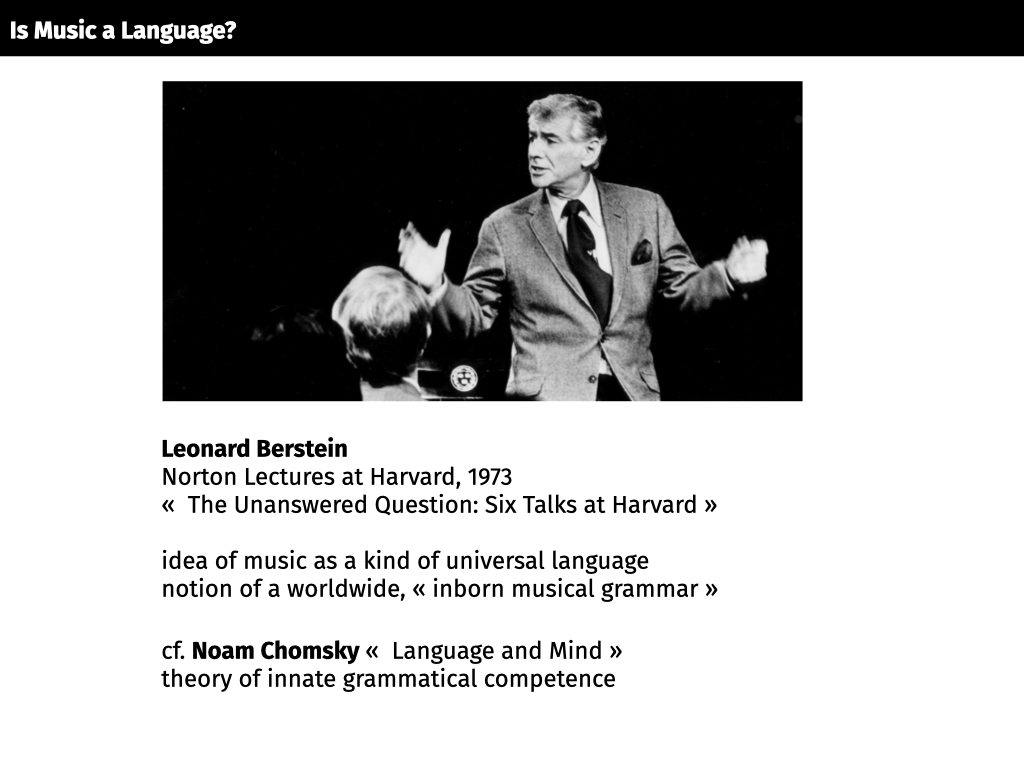
\includegraphics[height=85mm, width=125mm]{z_images/1_automatic_transcription/Bernstein.png}
\end{figure}\\
Aborder la musique à travers le TAL nécessite une réflexion autour de la musique en tant que langage ainsi que la possibilité de comparer ce même langage avec les langues naturelles. Quelques travaux en neuroscience ont abordé la question, notamment par observation des processus cognitifs et neuronaux que les systèmes de traitement de ces deux langages avaient en communs. Dans le travail de Poulin-Charronnat et al. \cite{poulincharronnat:hal-01985213}, la musique est reconnue comme étant un système complexe spécifique à l’être humain dont une des similitudes avec les langues naturelles est l’émergence de régularités reconnues implicitement par le système cognitif. La question de la pertinence de l’analogie entre langues naturelles et langage musical a également été soulevée à l’occasion de projets de recherche en TAL. Keller et al. \cite{keller:hal-03279850} ont exploré le potentiel de ces techniques à travers les plongements de mots et le mécanisme d’attention pour la modélisation de données musicales. La question du sens d’une phrase musicale apparaît, selon eux, à la fois comme une limite et un défi majeur pour l’étude de cette analogie.\\\\
\textit{Ici, Digression sur la musicologie calculatoire vs linguistique computationnelle ?}\\\\
D’autres travaux très récents, ont aussi été révélés lors de la \textit{première conférence sur le NLP pour la musique et l'audio (NLP4MusA 2020)}. Lors de cette conférence, Jiang et al. \cite{Jiang2020DiscoveringMR} ont présenté leur implémentation d’un modèle de langage musical auto-attentif visant à améliorer le mécanisme d'attention par élément, déjà très largement utilisé dans les modèles de séquence modernes pour le texte et la musique.\\
Il semblerait que le domaine du TAL qui se rapproche le plus du MIR serait la reconnaissance de la parole. En effet, la séparation des sources ont des approches similaires dans les deux domaines. De plus, il y a un lien entre partition musicale comme manière d’écrire la musique et texte comme manière d’écrire la parole.\\
Similitudes :\\
Reconnaissance automatique de la parole :\\
signal $\Rightarrow$ phonèmes $\Rightarrow$ texte
Transcription automatique de la musique :\\
signal $\Rightarrow$ MIDI $\Rightarrow$ partition
Différence :\\
Texte (données linéaires) ≠ partition (données structurées hiérarchiques)
\section{La transcription automatique de la musique}
%\subsection{Transcription musicale}
En musique, la transcription\footnote{\url{https://en.wikipedia.org/wiki/Transcription_(music)}} est la pratique consistant à noter un morceau ou un son qui n'était auparavant pas noté et/ou pas populaire en tant que musique écrite, par exemple, une improvisation de jazz ou une bande sonore de jeu vidéo. Lorsqu'un musicien est chargé de créer une partition à partir d'un enregistrement et qu'il écrit les notes qui composent le morceau en notation musicale, on dit qu'il a créé une transcription musicale de cet enregistrement.\\
%\subsection{Automatisation}
L'objectif de la transcription automatique de la musique (AMT) \cite{article1} est de convertir la performance d'un musicien en notation musicale - un peu comme la conversion de la parole en texte dans le traitement du langage naturel. L’AMT a des intérêt multiples, notemment pour la transcription de solos ou encore pour la constitution de corpus musicologiques. Ces deux aspects sont valables dans n’importe quels domaines musicaux dans lequels les partitions seraient inexistantes. Par exemple, dans les domaines oraux ou d’improvisation qui manquent de partition (jazz, pop) \cite{article1}.\\
Comme déjà évoqué précédemment, il s’agit d’un problème ancien et difficile. C’est un « graal » de l’informatique musicale. En 1976, H. C. Longuet-Higgins \cite{first_one} évoquait déjà la représentation musicale en arbre syntaxique dans le but d’écrire automatiquement des partitions à partir de données audio en se basant sur un mimétisme psychologique de l’approche humaine. De même pour les chercheurs en audio James A. Moorer, Martin Piszczalski et Bernard Galler qui, en 1977\footnote{\url{https://en.wikipedia.org/wiki/Transcription_(music)}}, ont utilisé leurs connaissances en ingénierie de l’audio et du numérique pour programmer un ordinateur afin de lui faire analyser un enregistrement musical numérique de manière à détecter les lignes mélodiques, les accords et les accents rythmiques des instruments à percussion.\\
%\subsection{Le processus général}
La tâche de transcription automatique de la musique comprend deux activités distinctes : l'analyse d'un morceau de musique et l'impression d'une partition à partir de cette analyse.\\\\
%\subsection*{Exemple de sous-tâche dans la figure 1.1 remplace ARCHITECTURE}
La figure \ref{AMT_presentation} est une proposition de Benetos et Al. \cite{article1} qui représente l'architecture générale d'un système de transcription musicale. On y observe plusieurs sous-tâches de l’AMT :
\begin{itemize}
	\item La séparation des sources à partir de l’audio.
	\item Le système de transcription :
	\begin{itemize}
		\item Cœur du système :\\
		$\Rightarrow$ Algorithmes de détection des multi-pitchs et de suivi des \tab notes.\\
		Quatres sous-tâches optionnelles accompagnent ces algorithmes :
		\begin{itemize}
			\item identification de l'instrument ;
			\item estimation de la tonalité et de l'accord ;
			\item détection de l'apparition et du décalage ;
			\item estimation du tempo et du rythme.
		\end{itemize}
	\end{itemize}
	\item Apprentissage sur des modèles accoustiques et musicologiques.
	\item \textit{Optionnel :} Informations fournies de manière externe. Soit fournis en amont (genre, instruments,…), soit par interaction avec un utilisateur (infos sur une partition incomplète).
\end{itemize}
\begin{figure}[!h]
	\centering
	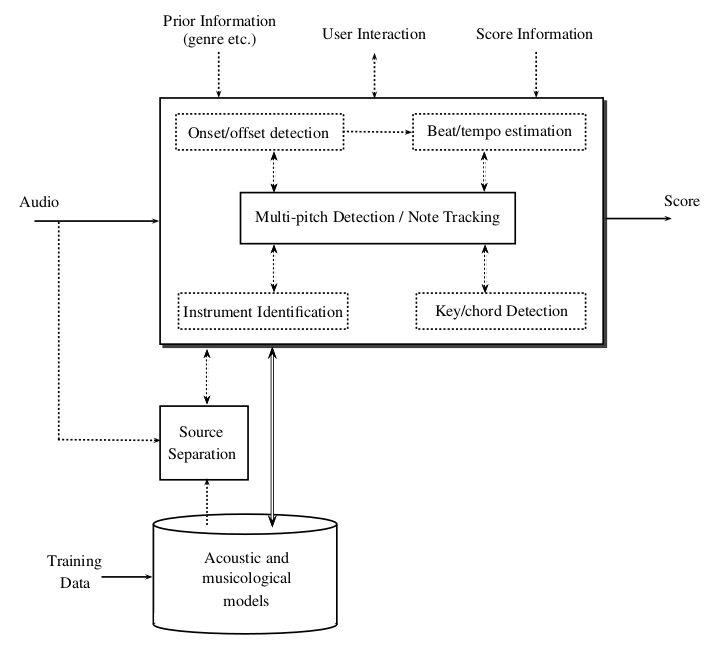
\includegraphics[height=95mm, width=130mm]{z_images/1_automatic_transcription/0_general_process.png}
	\caption{Transcription automatique}
	\label{AMT_presentation}
	\textit{Les sous-systèmes et algorithmes optionnels sont présentés à l'aide de lignes pointillées. Les doubles flèches mettent en évidence les connexions entre les systèmes qui incluent la fusion d'informations et une communication plus interactive entre les systèmes.}
\end{figure}\newpage
\section{La transcription automatique de la batterie}
La batterie est un instrument récent qui s’est longtemps passé de partition. En effet pour un batteur, la qualité de lecteur lorsqu’elle était nécessaire, résidait essentiellement dans sa capacité à lire les partitions des autres instrumentistes (par exemple, les grilles d’accords et la mélodie du thème en jazz) afin d’improviser un accompagnement approprié que personne ne pouvait écrire pour lui à sa place.\\
Les partitions de batterie sont arrivées par nécessité avec la pédagogie et l’émergence d’écoles de batterie partout dans le monde. Un autre facteur qui a contribué à l’expansion des partitions de batterie est l’arrivée de la musique assistée par ordinateur (MAO). En effet, l’usage de boîte à rythmes ou de séquenceurs permettant d’expérimenter soi-même l’écriture de rythmes en les écoutant mixés avec d’autres instruments sur des machines a permis  aux compositeurs de s’émanciper de la création d’un batteur en lui fournissant une partition contenant les parties exactes qu’ils voulaient entendre sur leur musique.\\
%\subsection{Utilité et problème de l’ADT}
La batterie a un statut à part dans l’univers de l’AMT puisqu'il s'agit d'instruments sans hauteur (du point de vue harmonique), d'événements sonores auxquels une durée est rarement attribuée et de notations spécifiques (symboles des têtes de notes).\\
Les applications de l’ADT seraient utiles dans tous les domaines musicaux contenant de la batterie mais aussi de manière plus générale dans le domaine du MIR. Si les ordinateurs étaient capables d'analyser la partie de la batterie dans la musique enregistrée, cela permettrait une variété de tâches de traitement de la musique liées au rythme. En particulier, la détection et la classification des événements sonores de la batterie par des méthodes informatiques est considérée comme un problème de recherche important et stimulant dans le domaine plus large de la recherche d'informations musicales \cite{8350302}.\\
\section{Les représentations de la musique}
\subsection*{Les données audio}
Le fichier WAV\footnote{https://en.wikipedia.org/wiki/WAV} est une instance du Resource Interchange File Format (RIFF) défini par IBM et Microsoft. Le format RIFF agit comme une "enveloppe" pour divers formats de codage audio.
Bien qu'un fichier WAV puisse contenir de l'audio compressé, le format audio WAV le plus courant est l'audio non compressé au format LPCM (linear pulse-code modulation). Le LPCM est également le format de codage audio standard des CD audio, qui stockent des données audio LPCM à deux canaux échantillonnées à 44 100 Hz avec 16 bits par échantillon. Comme le LPCM n'est pas compressé et conserve tous les échantillons d'une piste audio, les utilisateurs professionnels ou les experts en audio peuvent utiliser le format WAV avec l'audio LPCM pour obtenir une qualité audio maximale.
\subsection*{Les données MIDI}
Le MIDI\footnote{\url{https://en.wikipedia.org/wiki/MIDI}} (Musical Instrument Digital Interface) est une norme technique qui décrit un protocole de communication, une interface numérique et des connecteurs électriques permettant de connecter une grande variété d'instruments de musique électroniques, d'ordinateurs et d'appareils audio connexes pour jouer, éditer et enregistrer de la musique.\\\\
Les données midi sont représentées sous forme de piano-roll. Chaque points sur la figure \ref{piano_roll} est appelé « évènement midi » :
\begin{figure}[!h]
	\centering
	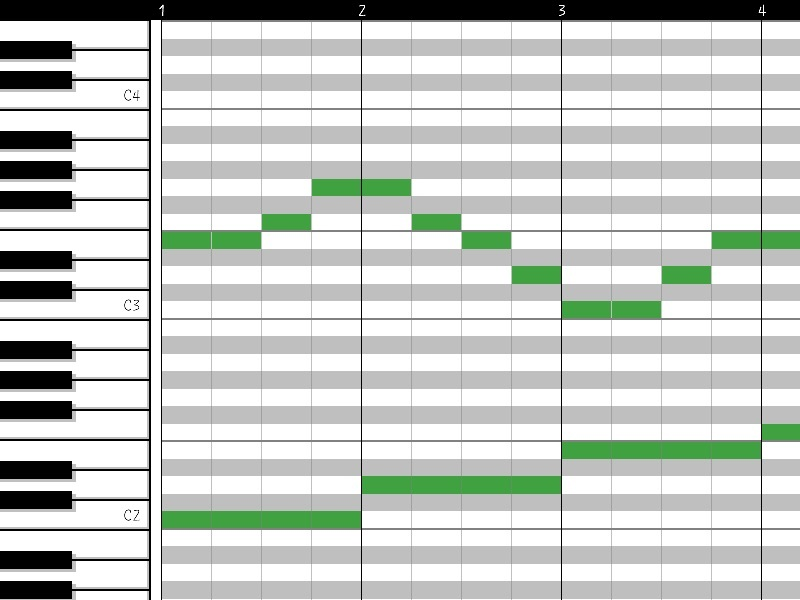
\includegraphics[height=40mm, width=50mm]{z_images/2_midi/exemple_midi_piano.jpg}
	\caption{Exemple évènements avec durée}
	\label{piano_roll}
\end{figure}\\
Chaque évènement MIDI rassemble un ensemble d’informations sur la hauteur, la durée, le volume, etc… :
\begin{figure}[h!]
	\centering
	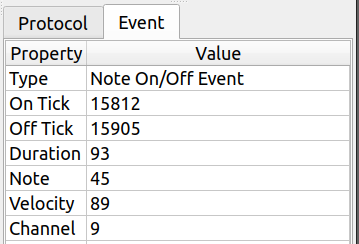
\includegraphics[height=40mm, width=50mm]{z_images/2_midi/representation_numerique_1.png}
	\caption{Critère pour un évènement}
\end{figure}\newpage
Pour la batterie, les évènements sont considérés sans durée, nous ignorerons donc les offsets (« Off Event »), les « Off Tick » et les « Duration ». Le channel ne nous sera pas utile non-plus.\\
\textit{Ici, définir Tick et channel.}\\\\
Voici un exemple de piano-roll midi pour la batterie :
\begin{figure}[h!]
	\centering
	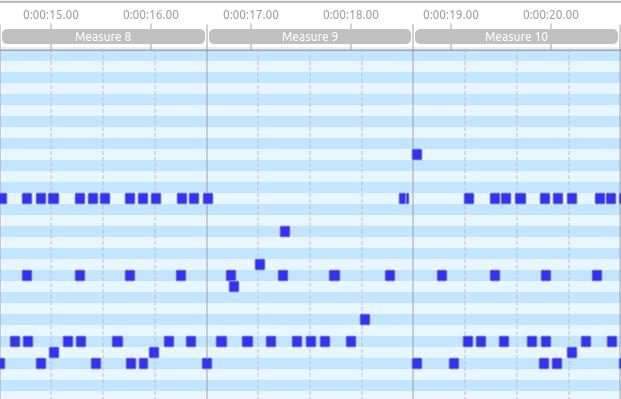
\includegraphics[height=40mm, width=50mm]{z_images/2_midi/representation_numerique_0.png}
	\caption{Exemple évènements sans durée}
\end{figure}\\
On observe que toutes les durées sont identiques.
\subsection*{Les partitions}
\begin{figure}[h!]
	\centering
	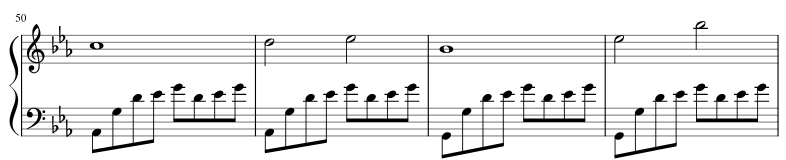
\includegraphics[height=30mm, width=120mm]{z_images/1_automatic_transcription/exemple_partoche.png}
	\caption{Exemple de partition de piano}
\end{figure}
Une partition de musique\footnote{\url{https://fr.wikipedia.org/wiki/Partition\_(musique)}} est un document qui porte la représentation systématique du langage musical sous forme écrite. Cette représentation est appelée transcription et elle sert à traduire les quatre caractéristiques du son musical :
\begin{itemize}
	\item la hauteur ;
	\item la durée ;
	\item l'intensité ;
	\item le timbre.
\end{itemize}
Ainsi que de leurs combinaisons appelées à former l'ossature de l'œuvre musicale dans son déroulement temporel, à la fois :
\begin{itemize}
	\item diachronique (succession des instants, ce qui constitue en musique la mélodie) ;
	\item et synchronique (simultanéité des sons, c'est-à-dire l'harmonie).
\end{itemize}
\section*{Conclusion}
Dans ce chapitre, nous avons établi que le MIR s’intéresse de plus en plus au TAL, et que par ce biais, il y a des liens possibles entre le langage musical et les langues naturelles, le plus proche étant probablement le phénomène d’écriture des sons de l’un comme l’autre.\\
Nous avons également établi que le MIR est né de l’AMT qui est un problème ancien et très difficile et qu’il serait toujours très utile de le résoudre (autant pour l’AMT que pour l’ADT).\\
Et enfin, nous avons décrit les représentations de la musique nécessaires à la compréhension du présent mémoire, allant du son jusqu’à l’écriture.

\chapter{État de l’art}
\label{chap:articles}
\minitoc
\section*{Introduction}
Dans ce chapitre, nous observerons les différentes avancées qui ont déjà eues lieues dans le domaine de la transcription automatique de la musique et de la batterie afin de situé notre démarche.\\
Nous aborderons le passage crucial du monophonique au polyphonique dans la transcription. Nous ferons un point sur les deux grandes parties de l’AMT de bout en bout : de l’audio vers le MIDI puis des données MIDI vers l’écriture d’une partition. Ensuite, nous ferons une critique des approches linéaires et des approches hiérarchiques. Enfin, nous ferons un bilan afin de situer l’ADT dans l’état de l’art de l’AMT.
\section{Monophonique et Polyphonique}
Les premiers travaux ont été faits sur l’identification des instruments monophoniques\footnote{Une seule note à la fois, ou plusieurs notes de même durée (monophonie par accord).}\cite{future_directions}. Actuellement, le problème de l'estimation automatique de la hauteur des signaux monophoniques peut être considéré comme résolu, mais dans la plupart des contextes musicaux, les instruments sont polyphoniques.\\
L'estimation des hauteurs multiples (détection multi-pitchs ou F0 multiples) est le problème central de la création d'un système de transcription de musique polyphonique. Il s’agit de la détection de notes qui peuvent apparaître simultanément et être produites par plusieurs instruments différents. Ce défi est donc majeur pour la batterie puisque c’est un instrument qui est lui-même constitué de plusieurs instruments.\\
Le fort degrés de chevauchement entre les durées ainsi qu’entre les fréquences complique l’identification des instruments polyphoniques. Cette tâche est étroitement liées à la séparation des sources et concerne aussi la séparation des voix. Les performances des systèmes actuels ne sont pas encore suffisantes pour permettre la création d'un système automatisé capable de transcrire de la musique polyphonique sans restrictions sur le degré de polyphonie ou le type d'instrument. Cette question reste donc encore ouverte. 
\section{Audio vers MIDI}
Utilité de l’audio vers MIDI dans la vraie vie $\Rightarrow$ p. 4 et 5 de \cite{Review_ADT}.\\\\
La plupart des travaux se sont concentrés sur le traitement du signal vers la génération du midi \cite{AMT_for_2_Instru}. Cette partie englobe plusieurs sous-tâches dont la détection multi-pitchs, la détection des onset et des offset, l'estimation du tempo, la quantification du rythme, la classification des genres musicaux,…\\
En ADT\cite{Review_ADT}, plusieurs stratégies de répartition Pre/Post-processing sont possibles pour la détection multi-pitchs. Une des démarches intuitives serait de la préparer dès le préprocessing, dans le pré-traitement, pendant la séparation des sources en supprimant les features non-pertinentes pour une meilleure détection des instruments de la batterie. Par exemple, en supprimant la structure harmonique pour atténuer l’influence des instruments à hauteurs sur la détection grosse-caisse et caisse-claire. Mais certaines études montrent que des expériences similaires ont donné des résultats non-concluants et que la suppression des instruments à hauteurs peut avoir des effets néfastes sur les performances de l’ADT. Cependant, les systèmes d’ADT basés sur des RNN ou des NMF font la séparation des sources pendant l’optimisation ce qui réduit la nécessité de la faire pendant le préprocessing.\\
Pour la reconnaissance des instruments, une approche possible\cite{Eronen} est de mettre un modèle probabiliste dans l’étape de la classification des évènements afin de classer les différents sons de la batterie. Dans cette méthode, on se place de sample audio isolés en modélisant la progression temporelle des features avec un HMM. Les features sont transformés en représentations statistiques indépendantes.
L’approche AdaMa\cite{adama_1} est une autre approche de la même catégorie, elle commence par une estimation initiale des sons de la batterie qui sont itérativement raffinés pour matcher l’enregistrement visé.\\
- Extraction of rhythmic information (tempo, beat, and musical timing)\\
\section{MIDI vers partition}
Lorsque les travaux principaux parlent de transcription de bout en bout, l’appellation « score » (\textit{partition}) désigne souvent un ouput au format Music XML, ou simplement MIDI. Par exemple, dans \cite{SHIBATA2021262}, la chaîne de traitement va jusqu’à la génération d’une séquence MIDI quantifiée qui est importée dans MuseScore pour en extraire manuellement un fichier MusicXML contenant plusieurs voix.\\
Seuls quelques travaux récents s’intéressent de près à la création d’outils permettant la génération de partition. Le problème de la conversion d'une séquence d'événements musicaux symboliques en une partition musicale structurée est traité notamment dans \cite{foscarin:hal-01988990}. Ce travail, qui vise à résoudre en une fois la quantification du rythme et la production de partition, s’appuie tout au long du processus sur  des grammaires génératives qui fournissent un modèle hiérarchique à priori des partitions. Les expériences ont des résultats prometteurs, mais il faut relevé qu’elle ont été menées avec un ensemble de données composé d'extraits monophoniques, il reste donc a traiter le passage au polyphonique en couplant le problème de la séparation des voix avec la quantification du rythme.\\
L'approche de \cite{foscarin:hal-01988990} est fondée sur la conviction que la complexité de la structure musicale dépasse les modèles linéaires.
\section{Approche linéaire et approche hiérarchique}
Plusieurs travaux ont d’abord privilégié l’approche stochastique. Par exemple, Shibata et al.\cite{SHIBATA2021262} ont utilisé le modèle de Markov caché (HMM)\footnote{\url{https://fr.wikipedia.org/wiki/Modèle_de_Markov_caché}}\footnote{\url{https://en.wikipedia.org/wiki/Hidden_Markov_model}} pour la reconnaissance de la métrique. Ils utilisent d’abord deux réseaux de neurones profonds, l’un pour la reconnaissance des pitchs et l’autre pour la reconnaissance de la vélocité. Pour la dernière couche, la probabilité est obtenue par une fonction sigmoïde. Ils construisent ensuite plusieurs HMM métriques étendus pour la musique polyphonique correspondant à des métriques possibles et ils calculent la probalitité maximale pour chaque modèle afin d’obtenir la métrique la plus probable.
\begin{figure}[h]
	\centering
	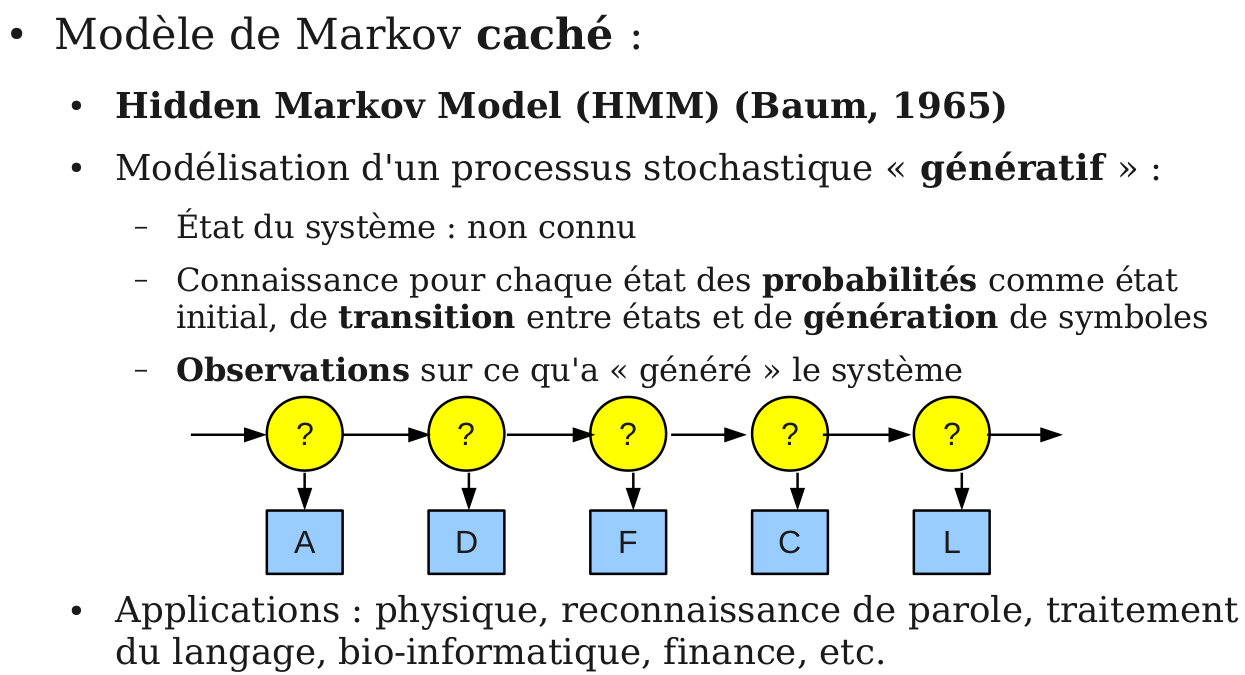
\includegraphics[height=50mm, width=90mm]{z_images/2_etat_de_l_art/hmm.png}
	\caption{HMM}
	\textit{Source : Cours de Damien Nouvel\footnote{\url{https://damien.nouvels.net/fr/enseignement}}}
\end{figure}
L’évaluation finale des résultats de \cite{SHIBATA2021262}, montre qu’il faut rediriger l’attention vers les valeurs des notes, la séparation des voix et d'autres éléments délicats de la partition musicale qui sont significatifs pour l'exécution de la musique. Hors, même si la quantification du rythme se fait le plus souvent par la manipulation de données linéaires allant notamment des real time units (secondes) vers les musical time units (temps, métrique,…), de nombreux travaux suggèrent d’utiliser une approche hiérarchique puisque le langage musical est lui-même structuré. En effet, ces structures (notamment les arbres syntaxiques) sont idéales pour représenter le langage musical.
Une méthodologie simple pour la description et l'affichage des structures musicales est présenté dans \cite{rythm_tree}. Les RT y sont évoqués comme permettant une cohésion complète de la notation musicale traditionnelle avec des notations plus complexes. Jacquemards et al.\cite{jacquemard:hal-01134096} propose aussi une représentation formelle du rythme sous forme d'arbre, inspirée de modèles théoriques antérieurs et dont l’objectif est la réécriture de termes. La réécriture d’arbres, dans un contexte de composition assistée par ordinateur par exemple, pourrait permettre de suggérer à un utilisateur diverses notations possibles pour une valeur rythmique, avec des complexités différentes. La nécessité d’une approche hiérarchique pour la production automatique de partition est évoquée dans \cite{foscarin:hal-01988990}. Les modèles de grammaire qui y sont exposés sont différents de modèles markoviens linéaires de précédent travaux.\newpage
\begin{figure}[h]
	\centering
	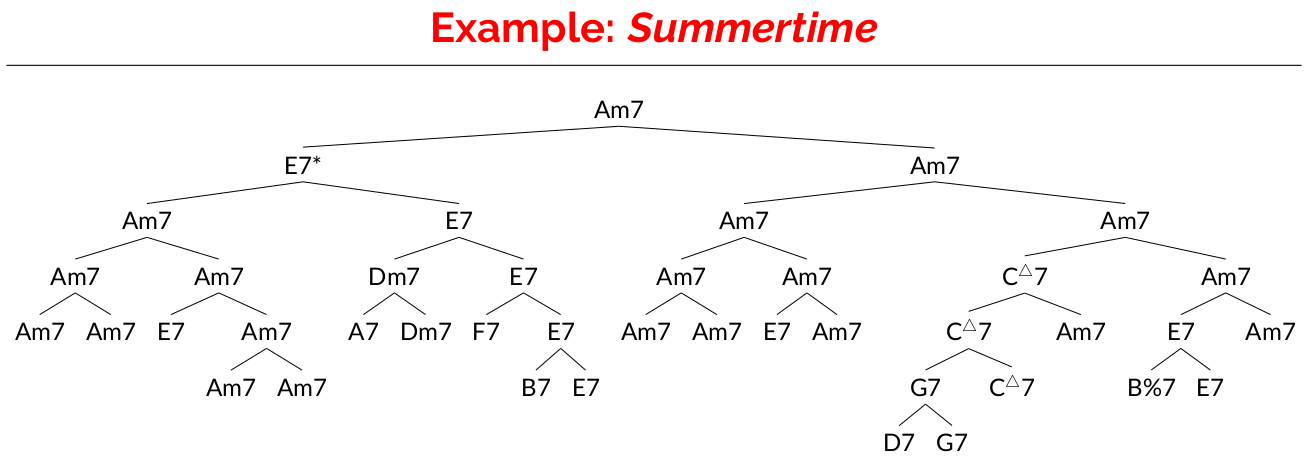
\includegraphics[height=40mm, width=120mm]{z_images/2_etat_de_l_art/summertime_tree.png}
	\caption{arbre\_jazz}
	\textit{Représentation arborescente d’une grille harmonique}\cite{harasimjazz}
\end{figure}
\section*{Conclusion}
\begin{itemize}
	\item Personne fait du MIDI vers partition ;
	\item Pas de formalisation de la notation de la batterie ;
	\item bla bla…
\end{itemize}
Un grand nombre travaux ont déjà été menés dans le domaine de l’ADT. La plupart ont été énumérés par Wu et al. \cite{Review_ADT} qui, pour mieux comprendre la pratique des systèmes d’ADT, se concentrent sur les méthodes basées sur la factorisation matricielle non négative et celles utilisant des réseaux neuronaux récurrents.\\
La plupart des travaux déjà entrepris se concentrent sur des méthodes de calcul pour la détection d'événements sonores de batterie à partir de signaux acoustiques ou sur la séparation entre les évènement sonore de batterie avec ceux des autres instruments dans un orchestre ou un groupe de musique \cite{2802}, ainsi que sur l'extraction de caractéristiques de bas niveau telles que la classe d'instrument et le moment de l'apparition du son. Très peu d'entre eux ont abordé la tâche de générer des partitions de batterie.
Nous avons décidé de compléter le travail qui concerne la batterie en commençant par l’endroit le moins pratiqué, à savoir la transcription du MIDI vers la partition.

\chapter{Méthodes}
\label{chap:07_methodes}
\minitoc
\section*{Introduction}
Dans ce chapitre, nous expliquerons en détail les méthodes que nous avons employées pour l’ADT.\\
Pour commencer, nous exposerons une description de la notation de la batterie ainsi qu’une modélisation de celle-ci pour la représentation des données rythmiques en arbres syntaxiques. Nous poursuiverons avec une présentation de qparse\footnote{https://qparse.gitlabpages.inria.fr/}, un outil de transcription qui est développé par Florent Jacquemard (Inria) au sein du laboratoire Cedric au CNAM.\\
Enfin, nous présenterons les systèmes. 
\section{La notation de la batterie}
\label{notation_batterie}
\begin{figure}[h]
	\centering
	
\includegraphics[height=10mm, width=25mm]{z_images/3_methodes/0_notation_de_la_batterie/0_figures_de_notes.png}
\end{figure}
Une figure de note \cite{danhauser} de musique combine plusieurs critères\footnote{\url{https://fr.wikipedia.org/wiki/Note_de_musique}} :
\begin{itemize}
	\item Une tête de note :\\
	Sa position sur la portée indique la hauteur de la note. La tête de note peut aussi indiquer une durée.
	\item Une hampe :\\
	Indicatrice d’appartenance à une voix en fonction de sa direction et indicatrice d’une durée représentée par sa présence ou non (blanche ≠ ronde)
	\item Un crochet : La durée d’une note est divisée par deux à chaque crochet ajouté à la hampe d’une figure de note.
\end{itemize}
\begin{figure}[h]
	\centering
	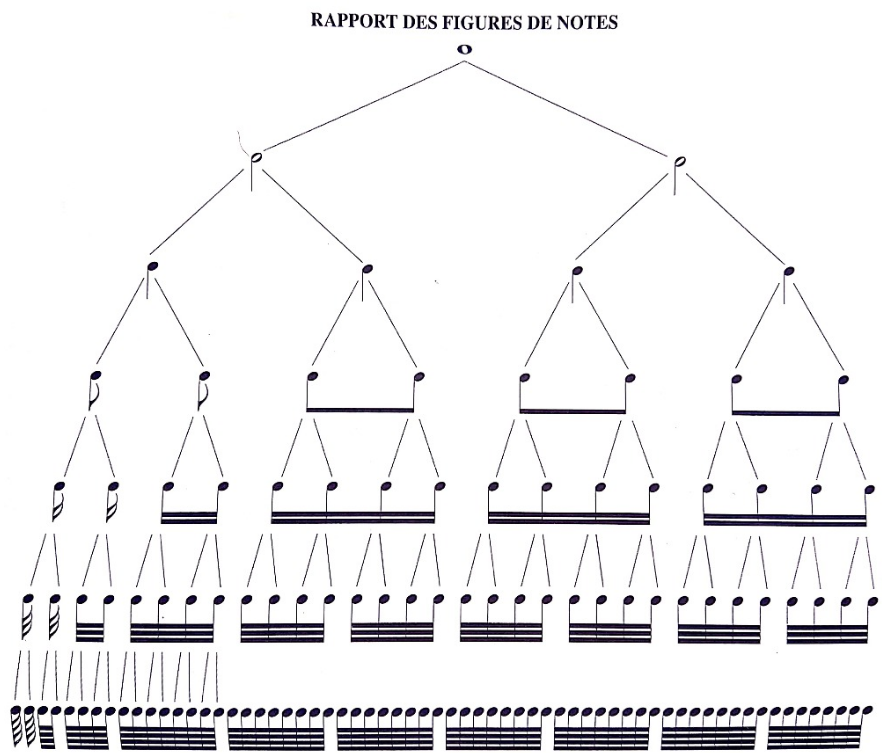
\includegraphics[height=50mm, width=80mm]{z_images/3_methodes/0_notation_de_la_batterie/1_rapport_figures_notes.png}
	\caption{Rapport des figures de notes}\cite{danhauser}
	\label{rapp_fig_notes}
\end{figure}
La figure \ref{rapp_fig_notes} montre les rapports de durée entre les figures de notes. Plus les durées sont longues, plus elles sont marquées par la tête de note (la note carrée fait deux fois la durée d’une ronde) ou la présence ou non de la hampe. À partir de la noire (3ème lignes en partant du haut), on ajoute un crochet à la hampe d’une figure de notes pour diviser sa durée par 2. Les notes à crochet (croche , double-croche, triple…) peuvent être reliées ou non par des ligatures (Voir les 4 dernière lignes de la figure \ref{rapp_fig_notes}).
\subsection*{Les hauteurs et les têtes de notes}
Pour la transcription, nous proposons une notation inspirée du recueil de pièces pour batterie de J.-F. Juskowiak \cite{jusko} et des méthodes de batterie Agostini \cite{ago_meth_3}, car nous trouvons la position des éléments cohérente et intuitive.\\
En effet, les hauteurs sur la portée représentent :
\begin{itemize}
	\item La hauteur physique des instruments :\\
	La caisse claire est centrale sur la portée et sur la batterie (au niveau de la ceinture, elle conditionne l’écart entre les pédales et aussi la position de tous les instruments basiques d’une batterie).\\
	Tout ce qui en-dessous de la caisse-claire sur la portée est en dessous de la caisse-claire sur la batterie (pédales, tom basse) ;\\
	Tout ce qui est au-dessus de la caisse-claire sur la portée, l’est aussi sur la batterie.\\
	\item La hauteur des instruments en terme de fréquences :\\
	Sauf pour le charley au pied et si l’on sépare en trois groupes (grosse-caisse, toms et cymbales), de bas en haut, les instruments vont du plus grave au plus aigu.
\end{itemize}
\begin{figure}[!h]
	\centering
	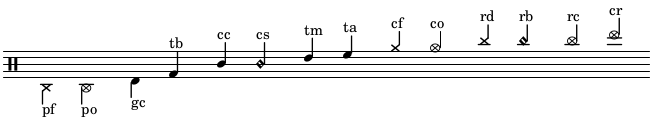
\includegraphics[height=25mm, width=130mm]{z_images/3_methodes/0_notation_de_la_batterie/2_hauteurs_et_tete_de_notes.png}
	\caption{Hauteur et têtes de notes}
	\label{Hauteur et têtes de notes}
\end{figure}
Les noms des instruments correspondant aux codes des notes de la figure \ref{Hauteur et têtes de notes} sont dans le tableau \ref{pitchs_instru}.
\subsection*{Les durées}
\label{hho}
Comme nous venons de la voir, la majorité des instruments de la batterie sont représentés par les têtes des notes. Par conséquent, les symboles rythmiques concernant la tête de note ne pourront pas être utilisés. Cela est valable aussi pour la présence ou non de la hampe puisque ce phénomène n’existe qu’avec les têtes de notes de type cercle-vide (opposition blanche-ronde). L’usage des blanches existe dans certaines partitions de batterie \cite{system_drums} mais cela reste dans des cas très rares. Certains logiciels permettent de faire des blanches avec des symboles spécifiques à la batterie ou aux percussions mais leur lecture reste peu aisée et leur utilisation pour la batterie est rarissime.\\
La durée d’une note peut être allongée par divers symboles :
\begin{itemize}
	\item Le point ;
	\item La liaison.
\end{itemize}
Ces symboles ne seront utiles que pour l’écriture des ouvertures de charley. Le charley est le seul instrument de la batterie dont la durée est quantitifiée (les cymbales attrapées à la main peuvent l’être aussi mais cela est très rare.)\newpage
\begin{figure}[h]
	\centering
	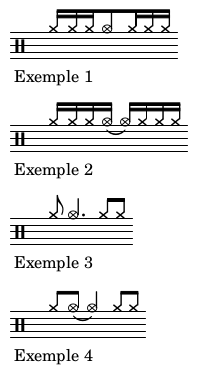
\includegraphics[height=80mm, width=40mm]{z_images/3_methodes/0_notation_de_la_batterie/3_point_et_liaison.png}
	\caption{Point et liaison}
	\label{point_liaison}
\end{figure}
L’écriture de la batterie doit faire ressortir la pulsation. La première chose à prendre en compte pour analyser la figure \ref{point_liaison} est donc la nécessité de regrouper les notes par temps à l’aide des ligatures.\\
Exemple 1 : ouverture de charley quantifiée mais pas notes pas regroupées par temps.\\
Exemple 2 : bieeen !\\
Exemple 3 et exemple 4 : les deux exemples sont valables mais le deuxième est le plus souvent utilisé car plus intuitif (regroupement par temps).\\
En cas de nécessité de rallonger la durée d’une note pour la batterie, on privilégiera la liaison.
\subsection*{Les silences}
\begin{figure}[h]
	\centering
	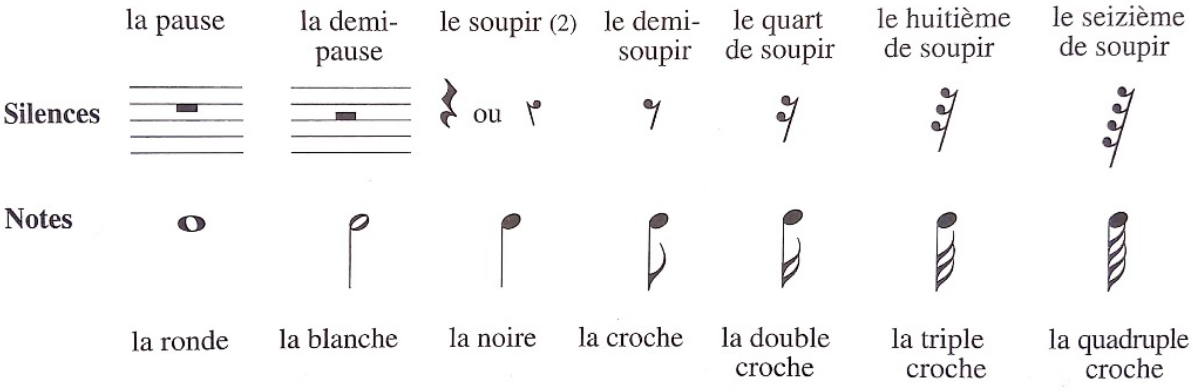
\includegraphics[height=35mm, width=120mm]{z_images/3_methodes/0_notation_de_la_batterie/4_silences.png}
	\caption{Les silences}
	\label{silences}
\end{figure}\newpage
Les silences sont parfois utilisés pour quantifier les ouvertures de charley. Les fermetures du charley sont notées soit par un silence (correspondant à une fermeture de la pédale), soit par un écrasement de l’ouverture par un autre coup de charley fermé, au pied ou à la main.
Physiquement, le charley est fermé par une pression du pied sur la pédale de charley. Dans les fichiers MIDI, cette pression est traduite par un charley joué au pied. Mais dans une vraie partition, cette écriture ne traduirait pas ce que le batteur doit penser.
\begin{figure}[h]
	\centering
	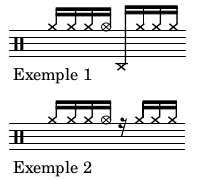
\includegraphics[height=40mm, width=40mm]{z_images/3_methodes/0_notation_de_la_batterie/5_silence_joue.png}
	\caption{Silence joué}
	\label{silence joue}
\end{figure}\\
L’exemple 1 de la figure \ref{silence joue} montre ce qui est écrit dans les données MIDI et l’exemple 2 montre ce que le batteur doit penser en lisant la partition. Il faut aussi prendre en compte l’écriture surchargée que l’exemple 1 donnerait avec une partition comprenant plusieurs voix et plusieurs instruments jouant simultanément.
\subsection*{Les équivalences rythmiques}
Pour les instruments mélodiques, la liaison et le point sont les deux seules possibilités en cas d’équivalence rythmique pour des notes dont la durée de l’une à l’autre est ininterrompue. Mais pour la batterie, à part pour les ouvertures de charley (voir section \ref{hho}), les durées des notes n’ont pas d’importance. L’usage des silences pour combler la distance rythmique entre deux notes devient donc possible.\\
Cela pris en compte, et étant donné que les indications de durée dans les têtes de notes sont peu recommandées (voir section \ref{hho}), l’écriture à l’aide de silences sera privilégiée comme indication de durée sauf dans les cas où cela reste impossible. Ce choix à pour but de n’avoir qu’une manière d’écrire toutes les notes, que leurs têtes de notes soit modifiées ou non.
\begin{figure}[h]
	\centering
	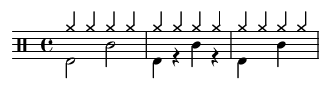
\includegraphics[height=20mm, width=75mm]{z_images/3_methodes/0_notation_de_la_batterie/6_equivalence.png}
	\caption{Équivalence}
	\label{equivalence}
\end{figure}\\
Sur la figure \ref{equivalence}, théoriquement, il faudra choisir la notation de la deuxième mesure mais dans certains contextes, pour des raisons de lisibilité ou de surcharge, la version sans les silences de la troisième mesure pourra être choisie.
\subsection*{Les voix}
Les voix\footnote{\url{https://fr.wikipedia.org/wiki/Voix_(polyphonie)}} désignent les différentes parties mélodiques constituant une composition musicale et destinées à être interprétées, simultanément ou successivement, par un ou plusieurs musiciens. En batterie, une voix est l’ensemble des instruments qui, à eux seuls, constituent une phrase rythmique et sont regroupés à l’aide des ligatures. Plusieurs écritures étant possibles pour un même rythme, on peut regrouper les instruments de la batterie par voix. Sur une portée de batterie, il existe le plus souvent 1 ou 2 voix. Sur la figure \ref{sep_voix}, il faudra faire un choix entre les exemples 1, 2 et 3 qui sont trois façons d’écrire le même rythme.
\begin{figure}[h]
	\centering
	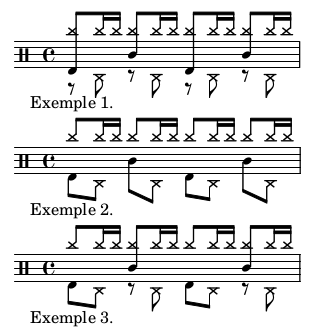
\includegraphics[height=65mm, width=60mm]{z_images/3_methodes/0_notation_de_la_batterie/7_voix.png}
	\caption{Séparation des voix}
	\label{sep_voix}
\end{figure}\\
Ce choix se fera en fonction des instruments joués, de la nature plus ou moins systèmatique de leurs phrasés, et des associations logiques entre les instruments dans la distribution des rythmes sur la batterie (voir la section \ref{sys_sep_voix}).
\subsection*{Les accentuations et les ghost-notes}
« Certaines notes dans une phrase musicale doivent, ainsi que les différentes syllabes d’un mot, être accentuées avec plus ou moins de force, porter une inflexion particulière. » \cite{danhauser}
\begin{figure}[h]
	\centering
	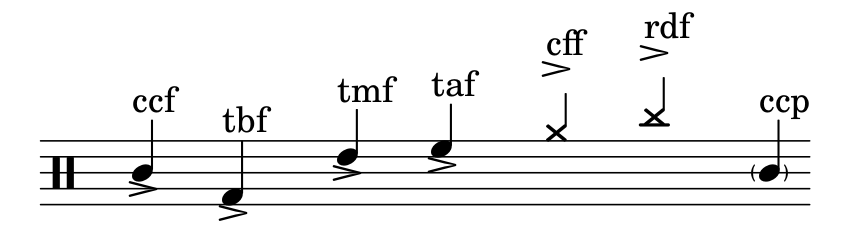
\includegraphics[height=25mm, width=75mm]{z_images/3_methodes/0_notation_de_la_batterie/8_nuances_0.png}
	\caption{Les accents et les ghost-notes}
	\label{accents_et_gn}
\end{figure}\\
La figure \ref{accents_et_gn} ne prend en compte que les accents que nous avons estimés nécessaires (voir la section \ref{velocite}). Les accents sont marqués par le symbole « > ». Il est positionné au-dessus des notes représentant des cymbales et en-dessous des notes représentant des toms ou la caisse-claire. Ce choix a été fait pour la partition de la figure \ref{partition_entiere} car elle est plus lisible ainsi, mais ces choix devront être adaptés en fonction des différents systèmes reconnus (voir la section \ref{systemes_methodes}). Par exemple, pour les systèmes jazz, les ligatures pour les toms et la caisse-claire seront dirigés vers le bas, il faudra donc mettre les symboles d’accentuation correspondants au-dessus des têtes de notes.\\
La dernière note de la figure \ref{accents_et_gn} montre un exemple de ghost-notes. Le parenthésage a été choisi car il peut être utilisé sur n’importe quelle note sans changer la tête de note.\\
Pour les codes, on prend le code de la note et on ajoute un « a » pour un accent et un « g » pour une ghost-note. Toutes les notes de la figure \ref{accents_et_gn} sont exposées en situation réelle dans la figure \ref{exemple_acc_et_gn}. 
\begin{figure}[h]
	\centering
	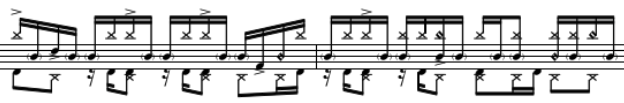
\includegraphics[height=20mm, width=110mm]{z_images/3_methodes/0_notation_de_la_batterie/8_nuances_1.png}
	\caption{Exemple pour les accentuations et les ghost-notes}
	\label{exemple_acc_et_gn}
\end{figure}\newpage
\section{Modélisation pour la transcription}
\label{modelisation_transcription}
\subsection*{Les pitchs}
\begin{table}[h]
	\centering
	\begin{tabular}{|c|c|c|} \hline
		Codes & Instruments & Pitchs \\ \hline
		cf & charley-main-fermé & 22, 42 \\
		co & charley-main-ouvert & 26 \\
		pf & charley-pied-fermé & 44 \\
		rd & ride & 51 \\
		rb & ride-cloche (bell) & 53 \\
		rc & ride-crash & 59 \\
		cr & crash & 55 \\
		cc & caisse-claire & 38, 40 \\
		cs & cross-stick & 37 \\
		ta & tom-alto & 48, 50 \\
		tm & tom-medium & 45, 47 \\
		tb & tom-basse & 43, 58 \\
		gc & grosse-caisse & 36 \\ \hline
	\end{tabular}
	\caption{Pitchs et instruments}
	\label{pitchs_instru}
\end{table}
Il existe, pour de nombreux instruments de la batterie, plusieurs samples audio associés à des pitchs. Pour cette première version, nous avons choisi de n’avoir qu’un code-instrument pour différentes variantes d’un instrument, c’est pourquoi certain code-instrument se voit attribuer plusieurs pitchs dans le tableau \ref{pitchs_instru}.\\
Malgré le large panel de pitchs disponible, il semblerait qu’aucun pitch ne désigne le charley ouvert joué au pied. Pourtant, dans la batterie moderne, plusieurs rythmes ne peuvent fournir le son du charley ouvert qu’avec le pied car les mains ne sont pas disponibles pour le jouer. Cela doit en partie être dû à l’utilisation des boîte à rythmes en MAO qui ne nécessitent pas de faire des choix conditionnés par les limitations humaines (2 pieds, 2 mains, et beaucoup plus d’instruments…)
\subsection*{La vélocité}
\label{velocite}
La partition de la figure \ref{partition_entiere} a été transcrite manuellement avec lilypond par analyse des fichiers MIDI et audio correspondants.\\
Cette transcription nous a mené aux observations suivantes :
\begin{itemize}
	\item Vélocité inférieure à 40 : ghost-note ;
	\item Vélocité supérieure à 90 : accent ;
	\item Pas d’intention d’accent ni de ghost-note pour une vélocité entre 40 et 89 ;
	\item Les accents et les ghosts-notes ne sont significatifs ni pour les instruments joués au pied, ni pour les cymbales crash.\\
	En effet, certaines vélocités en dessous de 40 étant détectées et inscrites dans les données MIDI sont dues au mouvement du talon du batteur qui bat la pulsation sans particulièrement jouer le charley. Ce mouvement est perçu par le capteur de la batterie électronique mais le charley n’est pas joué.
	\item Au final, nous avons relevé les ghost-notes et les accents pour la caisse-claire ainsi que les accents pour les toms et les cymbales rythmiques (charley et ride).
\end{itemize}
\subsection*{Les arbres de rythmes}
Les arbres de rythmes représentent un rythme unique dont les possibilités de notation sur une partition sont théoriquement multiples. Voici une représentation de la figure \ref{sep_voix} en arbre de rythmes avec les codes de chaque instrument :
\begin{figure}[h]
	\Tree[ [ [rd\\gc ][ [rd\\pf ][rd ]]]
	[ [rd\\cc ][ [rd\\pf ][rd ]]]
	[ [rd\\gc ][ [rd\\pf ][rd ]]]
	[ [rd\\cc ][ [rd\\pf ][rd ]]] ]
\end{figure}\\
Ci-dessous, le même arbre dont les codes des instruments sont remplacés par leurs données MIDI respectives :
\begin{figure}[h]
	\Tree[ [ [51\\36 ][ [51\\44 ][51 ]]]
	[ [51\\38 ][ [51\\44 ][51 ]]]
	[ [51\\36 ][ [51\\44 ][51 ]]]
	[ [51\\38 ][ [51\\44 ][51 ]]] ]
\end{figure}\\
Chacun des trois exemples de la figure \ref{sep_voix} est représenté par un des deux arbres syntaxiques ci-dessus.\newpage
\section{Qparse}
La librairie qparse\footnote{\url{https://qparse.gitlabpages.inria.fr}} implémente la quantification des rythmes basée sur des algorithmes d'analyse syntaxique pour les automates arborescents pondérés. En prenant en entrée une performance musicale symbolique (séquence de notes avec dates et durées en temps réel, typiquement un fichier MIDI), et une grammaire hors-contexte pondérée décrivant un langage de rythmes préférés, il produit une partition musicale. Plusieurs formats de sortie sont possibles, dont XML MEI.
Les principaux contributeurs sont :
\begin{itemize}
	\item Florent Jacquemard (Inria) : Développeur principal.
	\item Francesco Foscarin (PhD, CNAM) : Construction de grammaire automatique à partir de corpus ; Evaluation.
	\item Clement Poncelet (Salzburg U.) : Integration de la librairie Midifile pour les input MIDI.
	\item Philippe Rigaux (CNAM) : Production de partition au format MEI et de modèle intermédiaire de partition en sortie.
	\item Masahiko Sakai (Nagoya U.) : Mesure de la distance input/output pour la quantification et CMake framework. Évaluation.
\end{itemize}
\begin{figure}[h]
	\centering
	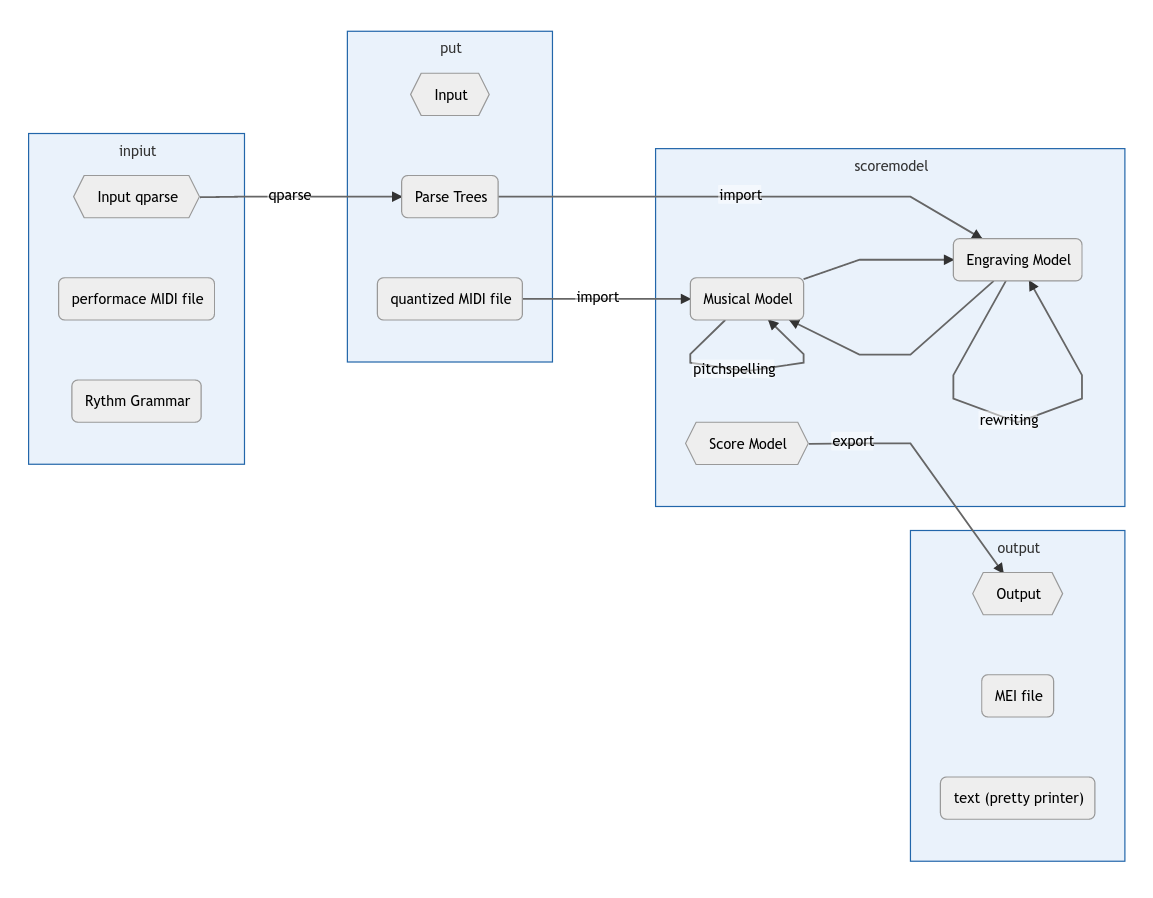
\includegraphics[height=95mm, width=130mm]{z_images/3_methodes/1_qparse/0_general_qparse.png}
	\caption{Présentation de qparse}
	\label{presentation_qparse}
\end{figure}
Explication des différentes étape de la figure \ref{presentation_qparse}\footnote{\url{https://gitlab.inria.fr/qparse/qparselib/-/tree/distance/src/scoremodel}} :
\begin{itemize}
	\item \textbf{Input Qparse} :\\
	Un fichier MIDI (séquence d’événements datés (piano roll) accompagné d’un fichier contenant une grammaire pondérée) ;
	\item \textbf{Parse Tree} :\\
	Les données MIDI sont quantifiées, les notes de dates proches sont alignées et les relation entre les notes sont identifiées (accords, fla, etc…). Un arbre de parsing global est créé ;
	\item \textbf{Score Model} :
	\begin{itemize}
		\item Les instruments sont identifiés dans scoremodel/import/tableImporterDrum.cpp ;
		\item Réécriture 1 :\\
		séparation des voix $\Rightarrow$ un arbre par voix $\Rightarrow$ représentation intermédiaire (RI) ;
		\item Réécriture 2 :\\
		simplification de l’écriture de chaque voix dans la RI ;
	\end{itemize}
    \item \textbf{Output} :\\
    export de la partition. Plusieurs formats sont possibles (xml, mei, lilypond,… ).\\
\end{itemize}
Plusieurs enjeux :
\begin{itemize}
	\item pb du MIDI avec qparse :\\
	ON-OFF en entrée $\Rightarrow$ 1 seul symbole en sortie.
	\item Minimiser la distance entre le midi et la représentation en arbre.
	\item Un des problèmes de Qparse était qu’il était limité au monophonique.\\
	Quelles sont les limites du monophonique ??
	\begin{itemize}
		\item Impossibilité de traiter plusieurs voix et de reconnaître les accords.
	\end{itemize}
\end{itemize}
\section{Les systèmes}
\label{systemes_methodes}
Un système est la combinaison d’un ou plusieurs éléments qui jouent un rythme en boucle (motif) et d’un autre élément qui joue un texte rythmique variable mais respectant les règles propres au système (gamme).
\subsection*{Définitions}
\textit{\textbf{Système :}} motif + gamme/texte\\
\textit{\textbf{Motif :}} rythmes coordonnés joués avec 2 ou 3 membres en boucle (reparti sur 1 ou 2 voix)\\
\textit{\textbf{Texte :}} rythme irrégulier joué avec un seul membre sur le motif (Réparti sur 1 voix).\\
\textit{\textbf{Gamme :}} La gamme d’un système considère l’ensemble des combinaisons que le batteur pourrait rencontrer en interprétant un texte rythmique à l’aide du système.\\\\
Un ensemble de systèmes comprenant leur métrique et leurs règles spécifiques de réécriture seront nécessaires. Il devront être distribué dans 4 grandes catégories :
\begin{table}[h]
	\centering
	\begin{tabular}{|c|c|c|c|c|} \hline
		Systèmes & Métriques & Subdivisions & Possibles & nb voix \\ \hline
		binaires & simple & doubles-croches & triolets, sextolets & 2 \\
		jazz & simple & triolets & croches et doubles-croches & 2 \\
		ternaires & complexe & croches & duolets, quartelets & 2 \\
		afros-cubains & simple & croches & - & 3 \\ \hline
	\end{tabular}
	\caption{Sytèmes}
\end{table}\\
Nous exposerons 3 systèmes afin d’illustrer les propos de cette section :
\begin{itemize}
	\item 4/4 binaire 
	\item 4/4 jazz
	\item 4/4 afro-cubain
\end{itemize}
\subsection*{Objectif des systèmes}
Les systèmes devront être matchés sur l’input MIDI afin de :
\begin{itemize}
	\item Définir une métrique ;
	\item Choisir une grammaire appropriée ;
	\item Fournir les règles de réécriture (séparation des voix et simplification.\\
\end{itemize}
La partie \textit{motif} des systèmes sera utilisée pour la \textbf{définition des métriques}. Le \textit{motif} et la gammes des systèmes sera utilisé pour la \textbf{séparation des voix}. Les règles de \textbf{simplification} (les combinaisons de réécritures) seront extraites des voix séparées des systèmes.
\subsubsection{Détection d’indication de mesure}
La détection de la métrique est importante non-seulement pour connaître le nombre de temps par mesure ainsi que le nombre de subdivision pour chacun de ces temps, mais aussi pour savoir comment écrire l’unité de temps et ses subdivisions.
\begin{figure}[h]
	\centering
	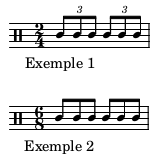
\includegraphics[height=40mm, width=40mm]{z_images/3_methodes/2_systemes/0_simple_VS_complexe.png}
	\caption{Métrique}
	\label{subdivisions}
\end{figure}\newpage
La figure \ref{subdivisions} montre deux indications de mesure différentes. L’une (exemple 1) est \textit{simple} (2 temps binaire sur lesquels sont joués des triolets), l’autre (exemple 2) est \textit{complexe} (2 temps ternaires). Le jazz est traditionnellement écrit en binaire avec ou sans triolet (même si cette musique est dite ternaire alors que le rock ternaire sera plutôt écrit comme dans l’exemple 2.
\subsubsection{Choix d’une grammaire}
Il faut prendre en compte l’existence potentielle de plusieurs grammaires chacunes dédiées à un type de contenu MIDI. Le choix d’une grammaire pondérée doit être fait avant le parsing puisque qparse prends en entrée un fichier MIDI et un fichier wta (grammaire). C’est pour cette raison que la métrique doit être définie avant le choix de la grammaire.\\
Pour les expériences effectuées avec le Groove MIDI Data Set, le style et l’indication de mesure sont récupérables par les noms des fichiers MIDI, mais il faudra par la suite les trouver automatiquement sans autres indications que les données MIDI elles-mêmes. Par conséquent, les motifs des systèmes devront être recherchés sur l’input \textit{(fichiers MIDI)} avant le lancement du parsing, afin de déterminer la métrique en amont. Cette tâche devra probablement être effectuée en Machine Learning.\newpage
\subsubsection{Séparation des voix}
\label{sys_sep_voix}
\begin{figure}[h]
	\centering
	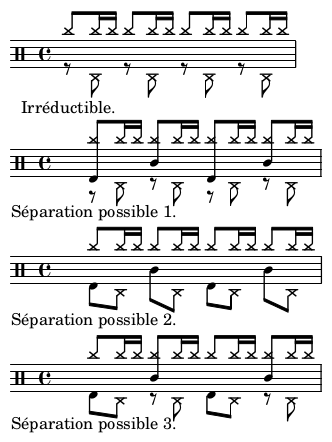
\includegraphics[height=60mm, width=40mm]{z_images/3_methodes/2_systemes/1_separation_4-4_binaire.png}
	\caption{Motif 4-4 binaire}
	\label{binaire}
\end{figure}
Ici, le système est construit sur un modèle rock en 4/4 : after-beat sur les 2 et 4 avec un choix de répartition des cymbales type fast-jazz. Le système est constitué par défaut du motif ride/ch-pf/cc et d’un texte joué à la grosse-caisse. La troisième séparation proposée est privilégiée car elle répartit selon 2 voix, une voix pour les mains (ride + cc) et une voix pour les pieds (ch-pf + gc). Ce choix paraît plus équilibré car deux instruments sont utilisés par voix et plus logique pour le lecteur puisque les mains sont en haut et les pieds en bas.\\

%D’autres choix d’écriture auraient été possibles :
%\begin{itemize}
%	\item Toutes les hampes en haut ;
%	\item Combinaison motif 1 et 2 en donnant 2 directions aux hampes de la cc).\\
%\end{itemize}
\begin{figure}[h]
	\centering
	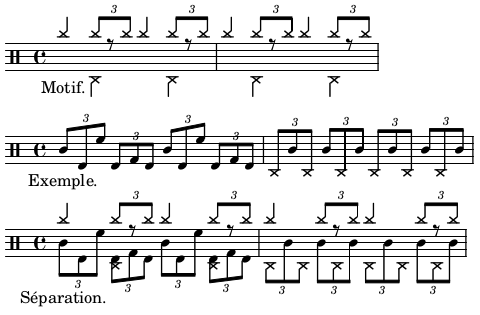
\includegraphics[height=45mm, width=60mm]{z_images/3_methodes/2_systemes/2_separation_4-4_jazz.png}
	\caption{Motif 4-4 jazz}
	\label{jazz}
\end{figure}
Dans la plupart des méthodes, le charley n’est pas écrit car il est considéré comme évident en jazz traditionnel. Ce qui facilite grandement l’écriture : la ride et les crash sur la voix du haut et le reste sur la voix du bas. Ici, le partie prit est de tout écrire. Dans l’exemple ci-dessus, les mesures 1 et 2 combinées avec le \textit{motif} de la première ligne, sont des cas typiques de la batterie jazz. Tout mettre sur la voix haute serait surchargé. De plus, la grosse caisse entre très souvent dans le flot des combinaisons de toms et de caisse claire et son écriture séparée serait inutilement compliquée et peu intuitive pour le lecteur. Le choix de séparation sera donc de laisser les cymbales en haut et toms, caisse-claire, grosse-caisse et pédale de charley en bas.
\begin{figure}[h]
	\centering
	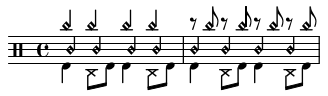
\includegraphics[height=20mm, width=70mm]{z_images/3_methodes/2_systemes/3_separation_afro-latins.png}
	\caption{Système 4-4 afro-latin}
	\label{afro_latin}
\end{figure}\\
La figure \ref{afro_latin} montre un exemple minimaliste de système afro-latins \cite{system_drums}. Ce système doit être écrit sur trois voix car la voix centrale est souvent plus complexe qu’ici (que des noirs) et la mélanger avec le haut ou le bas serait surchargé et peu lisible.
\subsubsection{Simplification de l’écriture}
Les gammes qui accompagnent les motifs d’un système étayent toutes les combinaisons d’un systèmes. Elles sont générées manuellement à partir de la simplification de chaque voix d’un système selon les principes de la section \ref{notation_batterie}. Aller à la section \ref{demo_sys} pour voir un exemple. 
\section*{Conclusion}
Nous avons formalisé une notation de la batterie, modélisé cette notation pour la transcription de données MIDI en partition, nous avons décrit qparse.\\
Enfin, nous exposé une approche de type dictionnaire (les « systèmes »)pour détecter une métrique, choisir une grammaire pondérée appropriée et énoncé des règles de séparation des voix et de simplification de l’écriture.

\chapter{Expérimentations}
\label{chap:08_experimentations}
\minitoc
\section*{Introduction}
Dans ce chapitre, nous présenterons le jeu de données et les analyses audio-MIDI. Nous ferons ensuite l’expérimentation théorique d’un \textit{système} implémentable qui devra être utilisé comme base de connaissances pour augmenter la rapidité et la qualité en sortie de Qparse. Enfin, nous présenterons les différentes contributions de développement.
\section{Le jeu de données}
Nous avons utilisé le Groove MIDI Dataset\footnote{\url{https://magenta.tensorflow.org/datasets/groove}} \cite{groove2019} (GMD) qui est un jeu de données mis à disposition par Google sous la licence Creative Commons Attribution 4.0 International (CC BY 4.0).\\
Le GMD est composé de 13,6 heures de batterie sous forme de fichiers MIDI et audio alignés. Il contient 1150 fichiers MIDI et plus de 22 000 mesures de batterie dans les styles les plus courants et avec différentes qualités de jeu. Tout le contenu a été joué par des humains sur la batterie électronique Roland TD-11 (figure \ref{electro_drums}).\newpage
\begin{figure}[h]
	\centering
	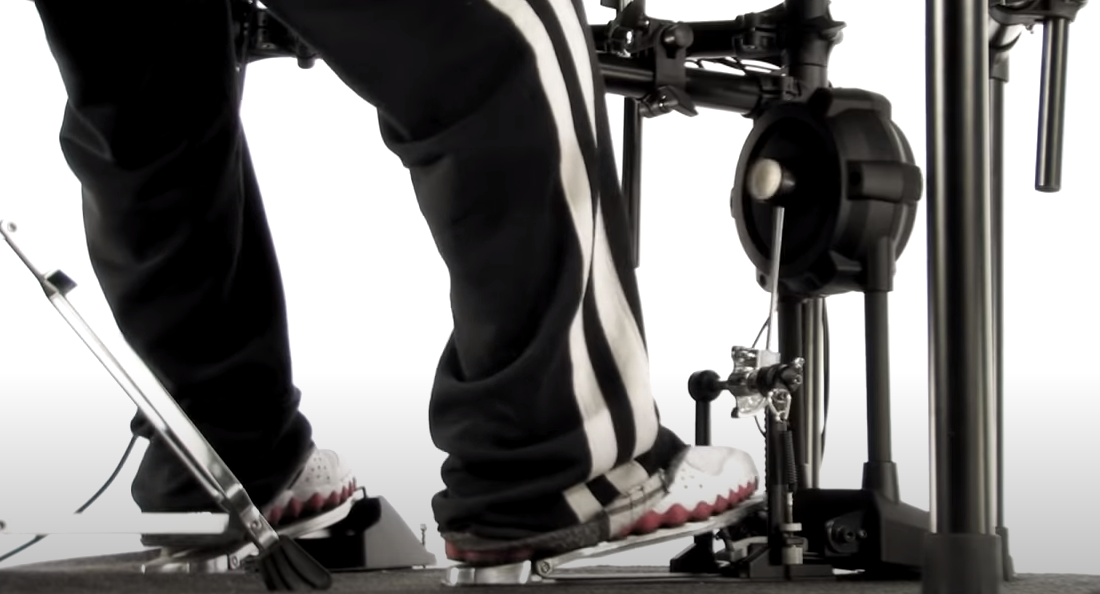
\includegraphics[height=35mm, width=60mm]{z_images/4_experimentations/0_groove/0_roland.png}\ \ 
	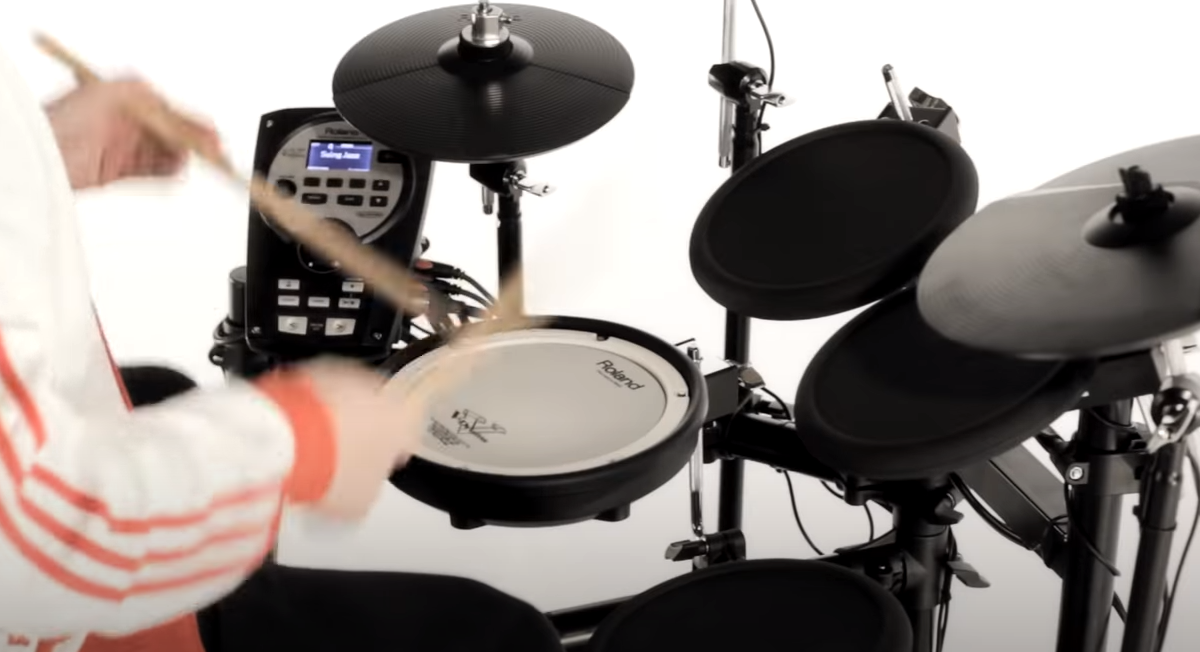
\includegraphics[height=35mm, width=60mm]{z_images/4_experimentations/0_groove/1_roland.png}
	\caption{Batterie électronique}
	\label{electro_drums}
	\textit{Source :} \url{https://www.youtube.com/watch?v=BX1V_IE0g2c}
\end{figure}
Autres critères spécifiques au GMD :
\begin{itemize}
	\item Toutes les performances ont été jouées au métronome et à un tempo choisi par le batteur.
	\item 80\% de la durée du GMD a été joué par des batteurs professionnels qui ont pu improviser dans un large éventail de styles. Les données sont donc diversifiées en termes de styles et de qualités de jeu (professionnel ou amateur).
	\item Les batteurs avaient pour instruction de jouer des séquences de plusieurs minutes ainsi que des fills\footnote{Un \textit{fill} est une séquence de relance dont la durée dépasse rarement 2 mesures. Il est souvent joué à la fin d’un cycle pour annoncer le suivant.}
	\item Chaque performance est annotée d’un style (fourni par le batteur), d’une métrique et d’un tempo ainsi que d’une identification anonyme du batteur.
	\item Il a été demandé à 4 batteurs d’enregistrer le même groupe de 10 rythmes dans leurs styles respectifs. Ils sont dans les dossiers eval-session du GMD.
	\item Les sorties audio synthétisées ont été alignées à 2 ms près sur leur fichier MIDI.
\end{itemize}
\subsection*{Format des données}
Le Roland TD-11 divise les données enregistrées en plusieurs pistes distinctes :
\begin{itemize}
	\item une pour le tempo et l’indication de mesure ;
	\item une pour les changements de contrôle (position de la pédale de charley) ;
	\item une pour les notes.\\
\end{itemize}
Les changements de contrôle sont placés sur le canal 0 et les notes sur le canal 9 (qui est le canal canonique pour la batterie).\\
Pour simplifier le traitement de ces données, ces trois pistes ont été fusionnées en une seule piste qui a été mise sur le canal 9.\\\\
« Control Changes
The TD-11 also records control changes specifying the position of the hi-hat pedal on each hit. We have preserved this information under control 4. »\\(\url{https://magenta.tensorflow.org/datasets/groove})\\$\Rightarrow$ ??? Je ne comprends pas encore comment trouver ce type d’informations dans les fichiers MIDI.\\L’utilisation de pretty\_midi devient urgente !
\section{Analyse MIDI-Audio}
\label{analyse_midi_audio}
Ces analyses ont été faites dans le cadre de transcriptions manuelles à partir de fichiers MIDI et Audio du GMD.
\subsection*{Comparaisons de transcriptions}
Pour les comparaisons de transcriptions, les transcriptions manuelles (TM) ont été éditées à l’aide de Lilypond\footnote{\url{http://lilypond.org/}} ou MuseScore\footnote{\url{https://musescore.com/}} et les transcriptions automatiques (TA) ont toutes été générées manuellement avec MuseScore.
\subsubsection{Exemple d’analyse 1}
\begin{figure}[h]
	\centering
	Transcription manuelle $\Rightarrow$ Transcription automatique
	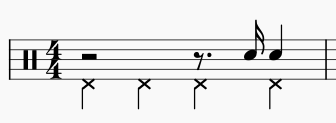
\includegraphics[height=20mm, width=50mm]{z_images/4_experimentations/1_analyse_midi_audio/0_drummer1_session3/1_manuelle.png}\ \ \ \ 
	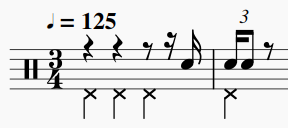
\includegraphics[height=20mm, width=45mm]{z_images/4_experimentations/1_analyse_midi_audio/0_drummer1_session3/0_musescore.png}
\end{figure}
\begin{itemize}
	\item Erreur d’indication de mesure (3/4 au lieu de 4/4) ;
	\item Les silences de la mesure 1 de la TA sont inutilement surchargés ;
	\item La noire du temps 4 de la mesure 1 de la TM est devenue les deux premières notes (une double-croche et une croche) d’un triolet sur le temps 1 de la mesure 2 de la TA.
\end{itemize}\newpage
\subsubsection{Exemple d’analyse 2}
\begin{figure}[h]
	\centering
	\tab Transcription manuelle $\Rightarrow$ Transcription automatique\\
	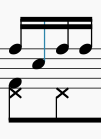
\includegraphics[height=20mm, width=13mm]{z_images/4_experimentations/1_analyse_midi_audio/0_drummer1_session3/5_manuelle.png}\ \ \ \ 
	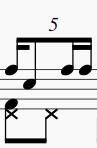
\includegraphics[height=20mm, width=13mm]{z_images/4_experimentations/1_analyse_midi_audio/0_drummer1_session3/4_musescore.png}
\end{figure}
\begin{itemize}
	\item Les doubles croches ont été interprétées en quintolet
	\item La deuxième double-croche est devenue une croche.\\
\end{itemize}
\subsubsection{Exemple d’analyse 3}
\begin{figure}[h]
	\centering
	Transcription manuelle $\Rightarrow$ Transcription automatique
	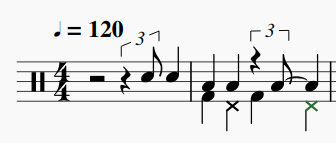
\includegraphics[height=24mm, width=50mm]{z_images/4_experimentations/1_analyse_midi_audio/0_drummer1_session3/3_manuelle.png}\ \ \ \ 
	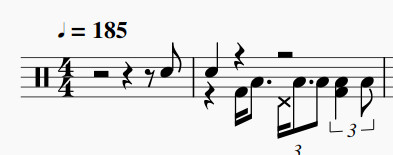
\includegraphics[height=25mm, width=55mm]{z_images/4_experimentations/1_analyse_midi_audio/0_drummer1_session3/2_musescore.png}
\end{figure}
\begin{itemize}
	\item Les grosses-caisses, les charleys et les caisses-claires ont été décalés d’un temps vers la droite.
	\item Les toms basses des temps 1 et 2 de la mesure 2 de la TM ont été décalés d’une double croche vers la droite dans la TA.
	\item La première caisse-claire de la mesure 1 devient binaire dans la TA alors qu’elle appartenait à un triolet dans la TM.
	\item Le triolet de tom-basse du temps 4 de la mesure 2 de la TA n’existe pas la TM.\\
\end{itemize}
\subsubsection{Exemple d’analyse 4}
\tab \tab Transcription manuelle $\Rightarrow$ Transcription automatique
\begin{figure}[h]
	\centering
	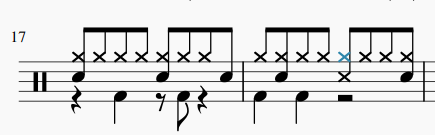
\includegraphics[height=19mm, width=50mm]{z_images/4_experimentations/1_analyse_midi_audio/1_drummer1_session1/3_manuelle.png}\ \ \ \ 
	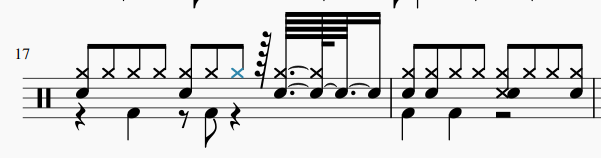
\includegraphics[height=19mm, width=70mm]{z_images/4_experimentations/1_analyse_midi_audio/1_drummer1_session1/2_musescore.png}
\end{figure}\\
Sur le temps 4 de la mesure 1, la deuxième croche a été transcrite d’une manière excessivement complexe !\newpage
\subsubsection{Exemple avec des flas}
Transcription manuelle\\
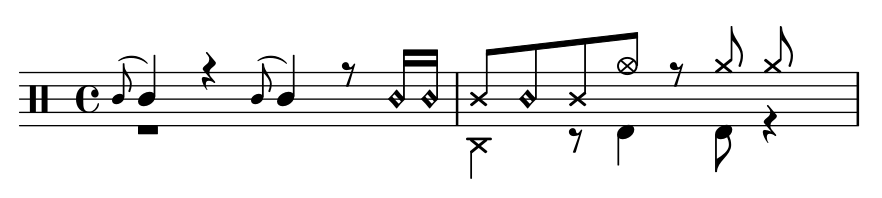
\includegraphics[height=25mm, width=95mm]{z_images/4_experimentations/1_analyse_midi_audio/2_transcriptions_flas/0_124_funk_95_fill_4-4.png}\\
Transcription automatique\\\\
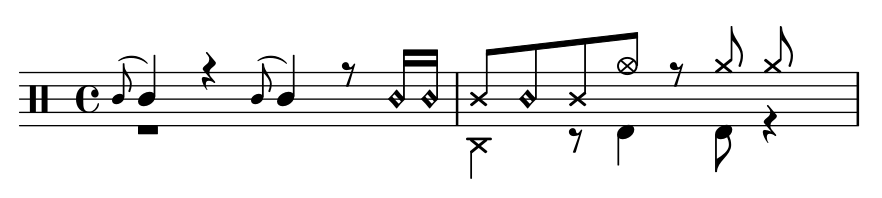
\includegraphics[height=20mm, width=130mm]{z_images/4_experimentations/1_analyse_midi_audio/2_transcriptions_flas/1_124_funk_95_fill_4-4.png}\\
\begin{itemize}
	\item Le premier fla est reconnu comme étant un triolet contenant une quadruple croche suivie d’une triple croche au lieu d’une seule note ornementée.
	\item Le deuxième fla est reconnu comme étant un accord.
	\item Les deux double en l’air sur le temps 4 de la TM sont mal quantifiée dans la TA. 
	\item La TA ne reconnaît qu’une mesure quand la TM en transcrit deux. En effet, la TA a divisé par deux la durée des notes afin de les faire tenir dans une mesure à 4 temps dont les unités de temps sont les noires. Par exemple, le soupir du temps 2 de la TM devient un demi-soupir sur le contre-temps du temps 1 dans la TA. Ou encore, la noire (pf, voir le tableau \ref{pitchs_instru}) sur le temps 1 de la mesure 2 de la TM suivie d’un demi-soupir devient une croche pointée sur le temps 3 de la TA.
	\item Autre problème : certaines têtes de notes sont mal attribuées. Par exemple, le charley ouvert en l’air sur le temps 2 de la mesure 2 de la TM devrait avoir le même symbole sur la TA. Idem pour les cross-sticks.
\end{itemize}\newpage
\subsection*{Transcription de partition}
\begin{figure}[h]
	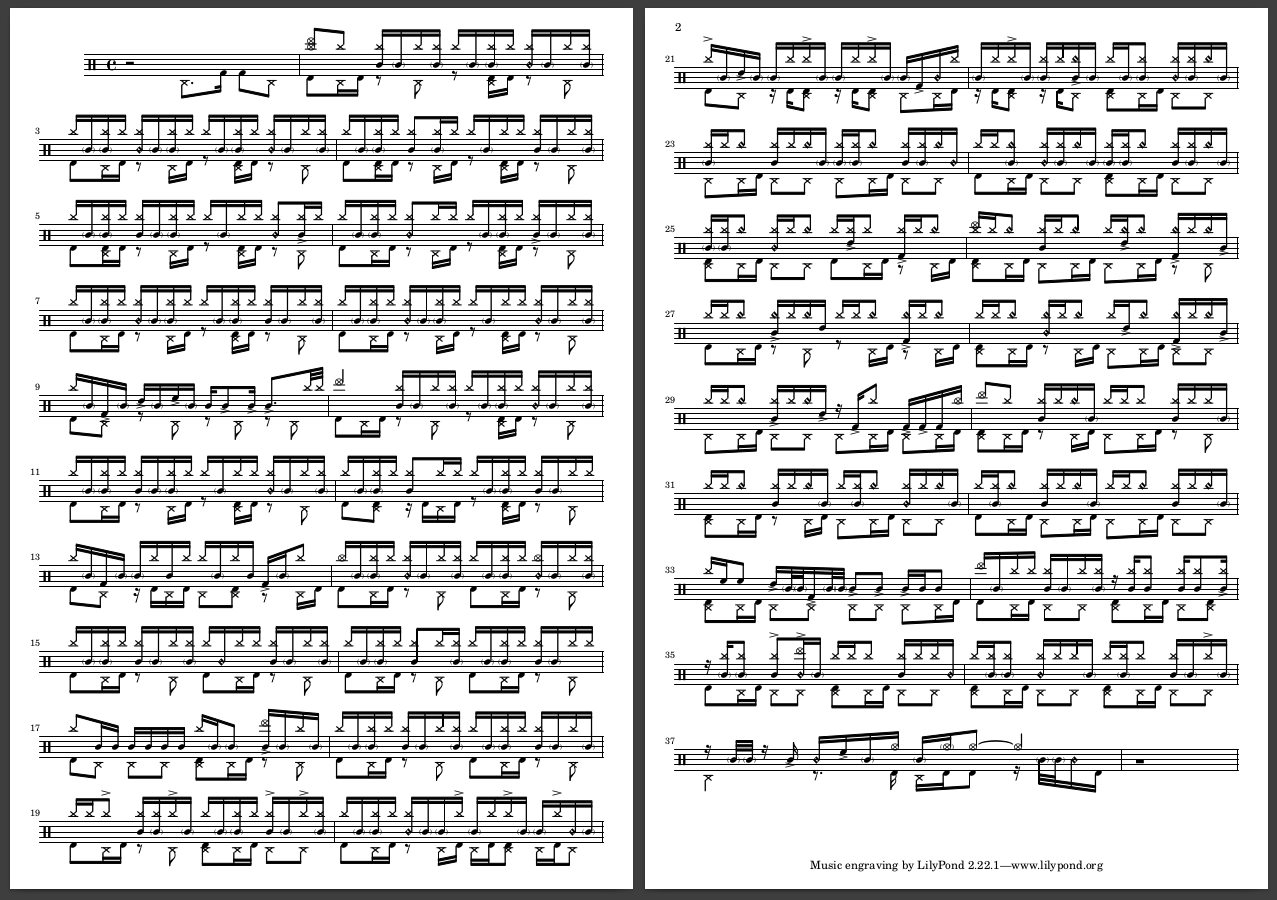
\includegraphics[height=120mm, width=160mm]{z_images/4_experimentations/1_analyse_midi_audio/3_partition.png}
	\caption{Partition entière}
	\label{partition_entiere}
\end{figure}
La figure \ref{partition_entiere} est la transcription manuelle des fichiers \textit{004\_jazz-funk\_116\_beat\_4-4.mid} et \textit{004\_jazz-funk\_116\_beat\_4-4.wav} du GMD.\\Cette transcription a été entièrement faite avec Lilypond (voir le code lilypond sur le git \url{https://github.com/MartinDigard/Stage_M2_Inria})
Il s’agit d’une partition d’un 4/4 binaire dont le fichier MIDI est annoncé dans le GMD de style «jazz-funk» probablement en raison de la ride de type shabada rapide (le ternaire devient binaire avec la vitesse) combiné avec l’after-beat de type rock (caisse-claire sur les deux et quatre).\\
La transcription des données audio et MIDI contenues dans ces fichiers a permis une analyse plus approndie des critères à relever pour chaque évènement MIDI et de la manière de les considérer dans un objectif de transcription en partition lisible pour un musicien (Voir la section \ref{modelisation_transcription}).
\section{Expérimentation théorique d’un système}
\subsection*{Motifs}
\begin{figure}[h]
	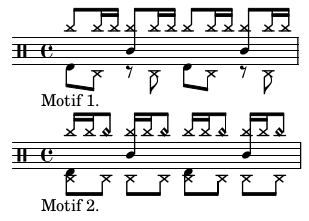
\includegraphics[height=30mm, width=40mm]{z_images/4_experimentations/2_demonstration_systeme/0_motifs_4-4_binaires.png}
	\caption{Motifs}
\end{figure}
Les motifs 1 et 2 peuvent être extraits de la figure 3.8. Ces deux motifs sont très classiques et seront réutilisables aussi dans d’autres contextes.\\
Le motif 1 est joué jusqu’à la mesure 18 avec des variations et des breaks.\\
Le motif 2 est joué des mesures 23 à 28.\\\\
\subsection*{Gammes}
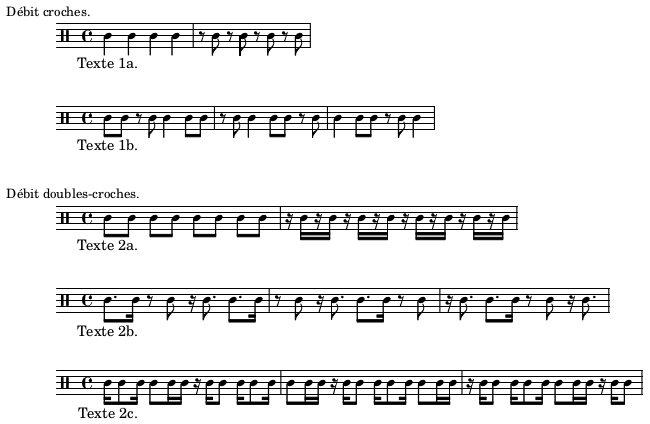
\includegraphics[height=70mm, width=95mm]{z_images/4_experimentations/2_demonstration_systeme/1_gammes_4-4_binaires.png}\\

\subsection*{Systèmes}
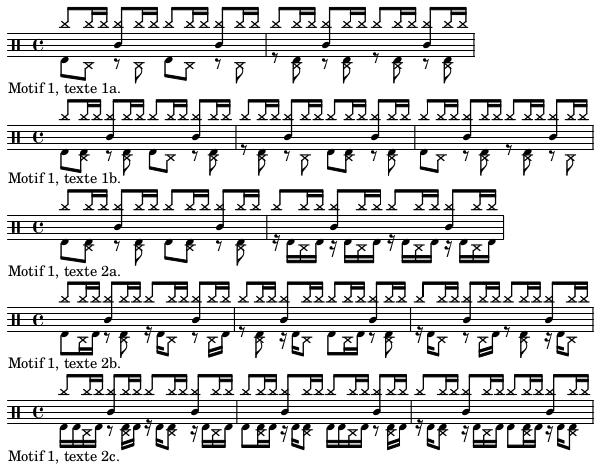
\includegraphics[height=75mm, width=85mm]{z_images/4_experimentations/2_demonstration_systeme/2_systeme_4-4_binaire.png}
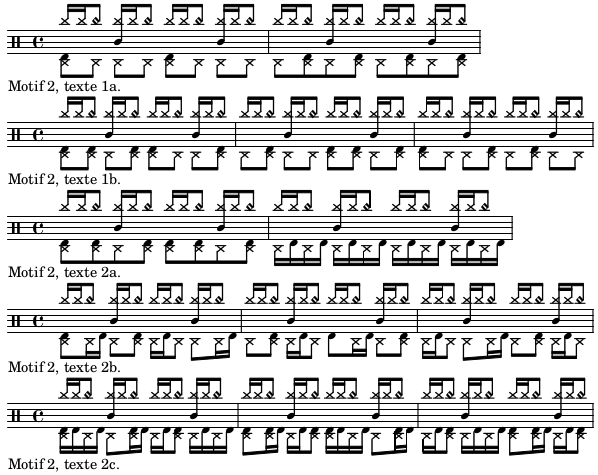
\includegraphics[height=75mm, width=85mm]{z_images/4_experimentations/2_demonstration_systeme/3_systeme_4-4_binaire.png}
\newpage

\subsection*{Démonstration}
\label{demo_sys}
\textbf{Représentation des systèmes en arbres de rythmes}

\resizebox{440pt}{!} {
	\Tree[.Motif\ 1\ +\ Texte\ 1a
	[.Mesure\ 1
	[.Temps\ 1 [rd\\bd ][ [rd\\pf ][rd ]]]
	[.Temps\ 2 [rd\\cc ][ [rd\\pf ][rd ]]]
	[.Temps\ 3 [rd\\bd ][ [rd\\pf ][rd ]]]
	[.Temps\ 4 [rd\\cc ][ [rd\\pf ][rd ]]] ]
	[.Mesure\ 2
	[.Temps\ 1 [rd ][ [rd\\bd\\pf ][rd ]]]
	[.Temps\ 2 [rd\\cc ][ [rd\\bd\\pf ][rd ]]]
	[.Temps\ 3 [rd ][ [rd\\bd\\pf ][rd ]]]
	[.Temps\ 4 [rd\\cc ][ [rd\\bd\\pf ][rd ]]] ]]}
\textbf{Réécriture}
\textit{Règles établies par le système}\\
\textbf{Séparation des voix}\\
\\\\
Ainsi l’arbre syntaxique de départ sera divisé en autant d’instruments qui le constituent et les voix seront regroupées de manière cohérentes.
\textit{Voix haute}\\
\resizebox{440pt}{!} {
	\Tree[.Motif\ 1\ +\ Texte\ 1a
	[.Mesure\ 1
	[.Temps\ 1 [rd ][ [rd ][rd ]]]
	[.Temps\ 2 [rd\\cc ][ [rd ][rd ]]]
	[.Temps\ 3 [rd ][ [rd ][rd ]]]
	[.Temps\ 4 [rd\\cc ][ [rd ][rd ]]] ]
	[.Mesure\ 2
	[.Temps\ 1 [rd ][ [rd ][rd ]]]
	[.Temps\ 2 [rd\\cc ][ [rd ][rd ]]]
	[.Temps\ 3 [rd ][ [rd ][rd ]]]
	[.Temps\ 4 [rd\\cc ][ [rd ][rd ]]] ]]}\\

\textit{Voix basse}\\
\resizebox{440pt}{!} {
	\Tree[.Motif\ 1\ +\ Texte\ 1a
	[.Mesure\ 1
	[.Temps\ 1 [bd ][ [pf ][t ]]]
	[.Temps\ 2 [t ][ [pf ][t ]]]
	[.Temps\ 3 [bd ][ [pf ][t ]]]
	[.Temps\ 4 [t ][ [pf ][t ]]] ]
	[.Mesure\ 2
	[.Temps\ 1 [t ][ [bd\\pf ][t ]]]
	[.Temps\ 2 [t ][ [bd\\pf ][t ]]]
	[.Temps\ 3 [t ][ [bd\\pf ][t ]]]
	[.Temps\ 4 [t ][ [bd\\pf ][t ]]] ]]}\\

\textbf{Règles de simplifications pour le 4/4 binaire}\\
Simplifier l’écriture de chaque voix (\textit{Règles établis par le système})\\
\resizebox{70pt}{!} {
	\Tree[.1/4 [t ][x ][x ][x ] ]
}\ \ \ \ \ $\Rightarrow$\ \ \ \ \
\resizebox{70pt}{!} {
	\Tree[.1/4 [r ][x ][x ][x ] ]
}\\\\

\resizebox{70pt}{!} {
	\Tree[.1/4 [x ][t ][x ][x ]]
}\ \ \ \ \ $\Rightarrow$\ \ \ \ \
\resizebox{50pt}{!} {
	\Tree[.1/4 [x ][ [x ][x ]]]
}\\\\

\resizebox{70pt}{!} {
	\Tree[.1/4 [t ][x ][x ][t ] ]
}\ \ \ \ \ $\Rightarrow$\ \ \ \ \
\resizebox{50pt}{!} {
	\Tree[.1/4 [ [r ][x ]][x ] ]
}\\\\

\resizebox{50pt}{!} {
	\Tree[.1/4 [t ][ [x ][x ]]]
}\ \ \ \ \ $\Rightarrow$\ \ \ \ \
\resizebox{50pt}{!} {
	\Tree[.1/4 [r ][ [x ][x ]]]
}\\\\

\resizebox{50pt}{!} {
	\Tree[.1/4 [t ][ [x ][t ]] ]
}\ \ \ \ \ $\Rightarrow$\ \ \ \ \
\resizebox{30pt}{!} {
	\Tree[.1/4 [r ][x ] ]
}\\\\

\resizebox{50pt}{!} {
	\Tree[.1/4 [x ][ [x ][t ]] ]
}\ \ \ \ \ $\Rightarrow$\ \ \ \ \
\resizebox{30pt}{!} {
	\Tree[.1/4 [x ][x ] ]
}
\section{Développement}
\subsection*{DrumCode}
Adaptation de la modélisation pour la transcription en cpp.
\subsection*{Tests unitaires sur les Jams}
\label{jam_tests}
Les Jams permettent de passer du monophonique au polyphonique.
\subsection*{Parsing}
\label{gram_pond}
Tests effectués avec le fichier midi suivant :\\\\
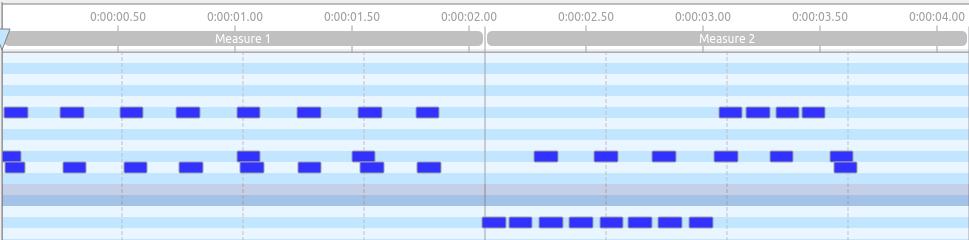
\includegraphics[height=50mm, width=160mm]{z_images/4_experimentations/3_developpement/0_midi_2bars_fill.png}\\\\
%\textit{Voix basse}\\
Un premier test convaincant est effectué avec la grammaire suivante :\\\\
// bar level\\
0 -> C0                1\\
0 -> E1                1\\
0 -> U4(1, 1, 1, 1)    1\\

// half bar level\\
9 -> C0                1\\
9 -> E1                1\\

// beat level\\
1 -> C0                1\\
1 -> E1                1\\
1 -> T2(2, 2)          1\\
1 -> T4(4, 4, 4, 4)    1\\

// croche level\\
2 -> C0                1\\
2 -> E1                1\\

// double level\\
4 -> C0                1\\
4 -> E1                1\\
4 -> E2                1\\
4 -> T2(6, 6)          1\\

// triple level\\
6 -> E1                1\\\\
Cette grammaire sépare les ligatures par temps au niveau de la mesure. Puis, au niveau du temps, elle autorise les divisions par deux (croches) et par quatre (doubles-croches). Tous les poids sont réglés sur 1. L’arbre de parsing en résultant est considéré comme « convaincant » car il découpe correctement les mesures et les temps.
\\\\
\resizebox{450pt}{!} {
\Tree[.Mesure\ 1
[.Temps\ 1 [0-ON\\1-ON\\2-ON ][3-OFF\\4-OFF\\5-OFF ][6-ON\\7-ON ][8-OFF\\9-OFF ]]
[.Temps\ 2 [10-ON\\11-ON ][12-OFF\\13-OFF ][14-ON\\15-ON ][16-OFF\\17-OFF ]]
[.Temps\ 3 [18-ON\\19-ON\\20-ON ][21-OFF\\22-OFF\\23-OFF ][24-ON\\25-ON ][26-OFF\\27-OFF ]]
[.Temps\ 4 [28-ON\\29-ON\\30-ON ][31-OFF\\32-OFF\\33-OFF ][34-ON\\35-ON ][36-OFF\\37-OFF ]]
]}\\\\\\
Les temps de la première mesure du fichier MIDI sont bien quantifié mais ceux de la deuxième mesure présentent quelques défauts de quantification visibles dès le premier temps.\\\\
\resizebox{300pt}{!} {
\Tree[.Mesure\ 2
[.Temps\ 1 [38-ON ][ [39-OFF ][40-ON ] ][ [41-OFF\\42-ON ][43-ON ] ][ [44-OFF\\45-OFF ][46-ON ] ]]
]}\\\\\\
Les Onsets sont correctement triés au niveau des doubles croches mais certaines doubles croches sont inutilement subdivisées en triples croches (les 2ème, 3ème et 4ème doubles croches sur le premier temps ci-dessus).\\\\
\textbf{2ème exemple :}\\
Après une augmentation du poids des triples croches dans la grammaire (monté de 1 à 5)et une baisse de tous les autres poids (descendu de 1 à 0.5), et mis à part le troisième temps de la 2ème mesure, tous les Onsets sont bien triés et aucuns ne sont subdivisés.






%\newpage
%\section{Résultats et discussion}
%\subsection{Résultats}
%\subsection{Évaluation}
%1 - Transcription manuelle à partir de fichier midi et/ou wav d’une partition contenant des systèmes. Écriture des systèmes contenues dans la partition (arbres, séparation des voix, réécriture)\\\\

\section*{Conclusion}
Conclusion de ce chapitre.

\chapter{Discussion}
\label{chap:09_discussion}
\minitoc
\section*{Introduction}
Dans ce chapitre, nous discuterons sur la pertinence de l’ensemble des choix qui ont été faits. Nous ferons un bilan des différentes avancées qui ont été faites ou non et nous tenterons d’en expliquer la ou les raisons.
\section{Travaux réalisés}
\textit{Faire une auto-critique des travaux réalisés.}
\subsection{Développer la notation}
\subsection{La modélisation}
\subsection{Le jeu de système}

\section{Travaux non-réalisés}
\textit{Expliquer pourquoi ces travaux n’ont pas pu être réalisés.}
\begin{itemize}
	\item implémenter un pattern…\\
	$\Rightarrow$ manque de temps ?\\
	\item La partie résultat est manquante car :\\
	$\Rightarrow$ Sujet très difficile ;\\
	$\Rightarrow$ Matcher les motifs peut être fait ultérieurement ;\\
	\tab Mais ce travail aurait été indispensable pour obtenir une quan-\tab tité de résultats qui justifieraient une évaluation automatique \tab permettant de faire des graphiques.\\
	\item L’évaluation fut entièrement manuelle car :\\
	$\Rightarrow$ Très dure automatiquement : il faut comparer 2 partitions (réf \tab VS output)
\end{itemize}
\section{Travaux futures}
\begin{itemize}
	\item Le ternaire jazz (voir expérience 2)
	\item Reconnaissance d’un motif sur le MIDI\\
	Reconnaître un motif (système) sur une mesure de l’input (un fichier midi représentant des données audios)\\
	$\Rightarrow$ Motif (système) reconnu : true ou false\\
	Si true :\\
	- Choisir la grammaire correspondante ;\\
	- Parser le MIDI ;\\
	- Appliquer les règles de réécritures (Séparation des voix et simplification)
\end{itemize}
\section*{Conclusion}
Sujet passionnant mais difficile. Obtenir la totalité des critères pour le mémoire n’aurait pas pu être fait sans bâcler. Une base solide spécifique à la batterie a été générée. Elle sera un bon point de départ pour les travaux futurs dont plusieurs propositions sont énoncés dans le présent document.


\cleardoublepage\pdfbookmark[-1]{Conclusion générale}{conclusion}
\chapter*{Conclusion générale}
\adjustmtc
\addstarredchapter{Conclusion générale}
Dans ce mémoire, nous avons traité de la problématique de la transcription automatique de la batterie. Son objectif était de transcrire, à partir de leur représentation symbolique MIDI, des performances de batteur de différents niveaux et dans différents styles en partitions écrites.\\
Nous avons avancé sur le parsing des données MIDI établissant un processus de regroupement des évènements MIDI qui nous a permis de faire la transition du monophonique vers le polyphonique. Une des données importante de ce processus était de différencier les nature des notes d’un \textit{accord}, notamment de distinguer lorsque 2 notes constituent un \textit{accord} ou un \textit{fla}.\\
Nous avons établis des \textit{grammaires pondérées} pour le parsing qui correspondent respectivement à des métriques spécifiques. Celles-ci étant sélectionnables en amont du parsing, soit par indication des noms des fichiers MIDI, soit par reconnaissance de la métrique avec une approche dictionnaire de patterns prédéfinis \footnote{\textit{Motifs} dans les \textit{systèmes} de la présente proposition.} qu’il serait pertinent de mettre en œuvre en machine learning.\\
Nous avons démontré que l’usage des \textit{systèmes} élimine un grand nombre de calcul lors de la réécriture. Pour la séparation des voix grâce au motif d’un système et pour la simplification grâce aux gammes du motif d’un système. Nous avons aussi montré comment, dans des travaux futurs, un système dont le motif serait reconnu en amont dans un fichier MIDI pourrait prédéfinir le choix d’une grammaire par la reconnaissance d’une métrique et ainsi améliorer le parsing et accélérer les choix ultérieurs dans la chaîne de traitement en terme de réécriture.\\
Il sera également intéressant d'étudier comment l'utilisation de LM peut améliorer les résultats de l'AM, voir [2], et ouvrir la voie à la génération entièrement automatisée de partitions de batterie et au problème général de l'AMT de bout en bout.\cite{future_directions}


%%%%%%%%%%%%%%%%%%%%%%%%%%%%%%%%%%%%%%%%%%%%%%%%%%%%%%%%%%%%%%%%%%%%%%%%%%%%%%%%%%
\cleardoublepage\pdfbookmark[-1]{Bibliographie}{bibliography}
\bibliographystyle{unsrt}
\bibliography{x_biblio}
\appendix
\cleardoublepage\pdfbookmark[-1]{Annexes}{appendix}
\include{z_annexe_lilypond}
\cleardoublepage
\pdfbookmark[-1]{Index}{index}
\printindex
\end{document}